\section{Introduction}

\emph{Rule lists}, also called decision lists, are one-sided decision trees.

\section{Related work}

\citep{rivest:1987}

\citep{LethamRuMcMa15}

\citep{YangRuSe16}

\citep{garofalakis:2000-kdd,garofalakis:2000-sigkdd,garofalakis:2003}

\section{A branch-and-bound framework for optimizing rule lists}

\subsection{Rule lists for binary classification}
\label{sec:setup}

We restrict our setting to binary classification,
where rule lists are Boolean functions;
this framework is straightforward to generalize to multi-class classification.
%
Let~${\{(x_n, y_n)\}_{n=1}^N}$ denote training data,
where ${x_n \in \{0, 1\}^J}$ are binary features and ${y_n \in \{0, 1\}}$ are labels.
%
Let~${\x = \{x_n\}_{n=1}^N}$ and~${\y = \{y_n\}_{n=1}^N}$,
and let~${x_{n,j}}$ denote the $j$-th feature of~$x_n$.

\begin{figure}[b!]
\begin{algorithmic}
\normalsize
\State \bif $p_1$ \bthen $q_1$
\State \belif $p_2$ \bthen $q_2$
\State \dots
\State \belif $p_K$ \bthen $q_K$
\State \belse $q_0$.
\end{algorithmic}
\caption{A $K$-rule list ${\RL = (r_1, r_2, \dots, r_K, r_0)}$, where
each rule ${r_k = p_k \rightarrow q_k}$, for all ${k = 0, \dots K}$.
We also equivalently write ${\RL = (\Prefix, \Labels, \Default, K)}$,
where ${\Prefix = (p_1, \dots, p_K)}$
and ${\Labels = (q_1, \dots, q_K)}$.}
\label{fig:rule-list}
\end{figure}

A rule list ${\RL = (r_1, r_2, \dots, r_K, r_0)}$ of length~${K \ge 0}$
is a ${(K+1)}$-tuple consisting of~$K$ distinct association rules,
${r_k = p_k \rightarrow q_k}$, for ${k = 1, \dots, K}$,
followed by a default rule~$r_0$.
%
Figure~\ref{fig:rule-list} illustrates~$\RL$,
which for clarity, we sometimes call a $K$-rule list.
%
An association rule~${r = p \rightarrow q}$ is an implication
corresponding to the conditional statement, ``if~$p$, then~$q$.''
%
In our setting, an antecedent~$p$ is a Boolean assertion that
evaluates to either true or false for each datum~$x_n$,
and a consequent~$q$ is a label prediction.
%
For example, ${(x_{n, 1} = 0) \wedge (x_{n, 3} = 1) \rightarrow (y_n = 1)}$
is an association rule.
%
%The number of conditions in an antecedent is its cardinality;
%the antecedent in the previous example has a cardinality of two.
%
The final default rule~$r_0$ in a rule list can be thought of
as a special association rule~${p_0 \rightarrow q_0}$
whose antecedent~$p_0$ simply asserts true.

Let ${\RL = (r_1, r_2, \dots, r_K, r_0)}$ be a $K$-rule list,
where ${r_k = p_k \rightarrow q_k}$ for each ${k = 0, \dots, K}$.
%
We introduce a useful alternate rule list representation:
${\RL = (\Prefix, \Labels, \Default, K)}$,
where we define ${\Prefix = (p_1, \dots, p_K)}$ to be $\RL$'s prefix,
${\Labels = (q_1, \dots, q_K) \in \{0, 1\}^K}$~gives
the label predictions associated with~$\Prefix$,
and we call ${\Default \in \{0, 1\}}$ the default label prediction.

Let ${\Prefix = (p_1, \dots, p_k, \dots, p_K)}$ be an antecedent list,
then for any~${k \le K}$, we define ${\Prefix^k = (p_1, \dots, p_k)}$
to be the $k$-prefix of~$\Prefix$.
%
For any such $k$-prefix~$\Prefix^k$,
we say that~$\Prefix$ starts with~$\Prefix^k$.
%
For any given space of rule lists,
we define~$\StartsWith(\Prefix)$ to be the set of
all rule lists whose prefixes start with~$\Prefix$:
\begin{align}
\StartsWith(\Prefix) =
\{(\Prefix', \Labels', \Default', K') : \Prefix' \textnormal{ starts with } \Prefix \}.
\end{align}
%We also say that an antecedent list~$\Prefix$ contains another
%antecedent list~$\Prefix'$ if the antecedents in~$\Prefix'$ correspond to
% a contiguous subsequence of antecedents anywhere in~$\Prefix$.

A rule list~$\RL$ classifies datum~$x_n$ by providing the label prediction~$q_k$
of the first rule~$r_k$ whose antecedent~$p_k$ is true for~$x_n$.
%
We say that an antecedent~$p_k$ of antecedent list~$\Prefix$ captures~$x_n$
in the context of~$\Prefix$ if~$p_k$ is the first antecedent in~$\Prefix$ that
evaluates to true for~$x_n$.
%
We also say that an antecedent list captures those data captured by its antecedents;
for a rule list~${\RL = (\Prefix, \Labels, \Default, K)}$,
data not captured by the prefix~$\Prefix$
are classified according to the default label prediction~$\Default$.

Let~$\beta$ be a set of antecedents.
%
We define~${\Cap(x_n, \beta) = 1}$ if an antecedent in~$\beta$
captures datum~$x_n$, and~0 otherwise.
%
For example, let~$\Prefix$ and~$\Prefix'$ be prefixes such that~$\Prefix'$ starts
with~$\Prefix$, then~$\Prefix'$ captures all the data that~$\Prefix$ captures:
\begin{align}
\{x_n: \Cap(x_n, \Prefix)\} \subseteq \{x_n: \Cap(x_n, \Prefix')\}.
\label{eq:cap-subset}
\end{align}
Now let~$\Prefix$ be an ordered list of antecedents,
and let~$\beta$ be a subset of antecedents in~$\Prefix$.
%
Let us define~${\Cap(x_n, \beta \given \Prefix) = 1}$ if~$\beta$
captures datum~$x_n$ in the context of~$\Prefix$,
\ie if the first antecedent in~$\Prefix$ that evaluates to true for~$x_n$
is an antecedent in~$\beta$,
and~0 otherwise.
%
Note that ${\Cap(x_n, \beta \given \Prefix) = 1}$ only if ${\Cap(x_n, \beta) = 1}$;
${\Cap(x_n, \beta \given \Prefix) = 0}$ either if ${\Cap(x_n, \beta) = 0}$,
or if ${\Cap(x_n, \beta) = 1}$ but there is an antecedent~$\alpha$ in~$\Prefix$,
preceding all antecedents in~$\beta$, such that ${\Cap(x_n, \alpha) = 1}$.
%
Now, define~${\Supp(\beta, \x)}$ to be the normalized support of~$\beta$,
\begin{align}
\Supp(\beta, \x) = \frac{1}{N} \sum_{n=1}^N \Cap(x_n, \beta),
\label{eq:support}
\end{align}
and similarly define~${\Supp(\beta, \x \given \Prefix)}$
to be the normalized support of~$\beta$ in the context of~$\Prefix$,
\begin{align}
\Supp(\beta, \x \given \Prefix) = \frac{1}{N} \sum_{n=1}^N \Cap(x_n, \beta \given \Prefix),
\label{eq:support-context}
\end{align}

Finally, we address how empirical data constrains rule lists.
%
Given training data~${(\x, \y)}$,
an antecedent list ${\Prefix = (p_1, \dots, p_K)}$
implies a rule list ${\RL = (\Prefix, \Labels, \Default, K)}$
with prefix~$\Prefix$, where the label predictions
${\Labels = (q_1, \dots, q_K)}$ and~$\Default$ are empirically set
to minimize the number of misclassification errors made by
the rule list on the training data.
%
Thus for~${1 \le k \le K}$, label prediction~$q_k$ corresponds to the
majority label of data captured by antecedent~$p_k$ in the context of~$\Prefix$,
and the default~$\Default$ corresponds to the majority label of data
not captured by~$\Prefix$.
%
In the remainder of our presentation, whenever we refer to a rule list with a
particular prefix, we implicitly assume these empirically determined label predictions.

\subsection{Branch-and-bound optimization framework}

We define a simple objective function for a rule list ${\RL = (\Prefix, \Labels, \Default, K)}$:
\begin{align}
\Obj(\RL, \x, \y) = \Loss(\RL, \x, \y) + \Reg K.
\label{eq:objective}
\end{align}
This objective function is a regularized empirical risk;
it consists of a loss~$\Loss(\RL, \x, \y)$ measuring misclassification error,
and a regularization term that penalizes longer rule lists.
%
$\Loss(\RL, \x, \y)$~is the fraction of training data whose labels are
incorrectly predicted by~$\RL$.
%
In our setting, the regularization parameter~${\Reg \ge 0}$ is a small constant;
\eg ${\Reg = 0.01}$ can be thought of as adding a penalty equivalent to misclassifying~$1\%$
of data when increasing a rule list's length by one association rule.
%
%As noted in~\S\ref{sec:setup}, a prefix~$\Prefix$ and training data together
%fully specify a rule list~${\RL = (\Prefix, \Labels, \Default, K)}$,
%thus let us define~${\Obj(\Prefix, \x, \y) \equiv \Obj(\RL, \x, \y)}$.

Our objective has structure amenable to global optimization via a branch-and-bound framework.
%
We can decompose the misclassification error into two contributions
corresponding to the prefix and default:
\begin{align}
\Loss(\RL, \x, \y) %= \Loss(\Prefix, r_q, \Default, \x, \y)
\equiv \Loss_p(\Prefix, \Labels, \x, \y) + \Loss_0(\Prefix, \Default, \x, \y),
\end{align}
where ${\Prefix = (p_1, \dots, p_K)}$ and ${\Labels = (q_1, \dots, q_K)}$;
\begin{align}
\Loss_p(\Prefix, \Labels, \x, \y) =
\frac{1}{N} \sum_{n=1}^N \sum_{k=1}^K \Cap(x_n, p_k \given \Prefix) \wedge \one [ q_k \neq y_n ]
\label{eq:loss}
\end{align}
is the fraction of data captured and misclassified by the prefix, and
\begin{align}
\Loss_0(\Prefix, \Default, \x, \y) =
\frac{1}{N} \sum_{n=1}^N \neg\, \Cap(x_n, \Prefix) \wedge \one [ \Default \neq y_n ]
\end{align}
is the fraction of data not captured by the prefix and misclassified by the default.
%
Eliminating the latter error term gives a lower bound~$b(\Prefix, \x, \y)$ on the objective,
\begin{align}
b(\Prefix, \x, \y) \equiv \Loss_p(\Prefix, \Labels, \x, \y) + \Reg K \le \Obj(\RL, \x, \y),
\label{eq:lower-bound}
\end{align}
where we have suppressed the lower bound's dependence on label predictions~$\Labels$
because they are fully determined, given~${(\Prefix, \x, \y)}$.
%
Furthermore, as we state next in Theorem~\ref{thm:bound},
$b(\Prefix, \x, \y)$ gives a lower bound on the objective of
\emph{any} rule list whose prefix starts with~$\Prefix$.

\begin{theorem}[Hierarchical objective lower bound]
Define~${b(\Prefix, \x, \y) = \Loss_p(\Prefix, \Labels, \x, \y) + \Reg K}$.
%
Also, define
${\StartsWith(\Prefix) = \{(\Prefix', \Labels', \Default', K') : \Prefix' \textnormal{ starts with } \Prefix \}}$
to be the set of all rule lists whose prefix starts with~$\Prefix$.
%
Let ${\RL = (\Prefix, \Labels, \Default, K)}$ be a rule list
with prefix~$\Prefix$, and let
${\RL' = (\Prefix', \Labels', \Default', K') \in \StartsWith(\Prefix)}$
be any rule list such that its prefix~$\Prefix'$ starts with~$\Prefix$
and ${K' \ge K}$, then ${b(\Prefix, \x, \y) \le \Obj(\RL', \x, \y)}$.
\label{thm:bound}
\end{theorem}

\begin{proof}
Let ${\Prefix = (p_1, \dots, p_K)}$ and ${\Labels = (q_1, \dots, q_K)}$;
let ${\Prefix' = (p_1, \dots, p_K, p_{K+1}, \dots, p_{K'})}$
and ${\Labels' = (q_1, \dots, q_K, q_{K+1}, \dots, q_{K'})}$.
%
Notice that~$\Prefix'$ yields the same mistakes as~$\Prefix$,
and possibly additional mistakes:
\begin{align}
\Loss_p(\Prefix', \Labels', \x, \y)
&= \frac{1}{N} \sum_{n=1}^N \left( \sum_{k=1}^K \Cap(x_n, p_k \given \Prefix) \wedge \one [ q_k \neq y_n ]
+ \sum_{k=K+1}^{K'} \Cap(x_n, p_k \given \Prefix') \wedge \one [ q_k \neq y_n ] \right) \nn \\
&\ge \Loss_p(\Prefix, \Labels, \x, \y),
\label{eq:prefix-loss}
\end{align}
where we have used the fact that
${\Cap(x_n, p_k \given \Prefix') = \Cap(x_n, p_k \given \Prefix)}$
for~${1 \le k \le K}$.
%
It follows that
\begin{align}
b(\Prefix, \x, \y) &= \Loss_p(\Prefix, \Labels, \x, \y) + \Reg K \nn \\
&\le  \Loss_p(\Prefix', \Labels', \x, \y) + \Reg K' = b(\Prefix', \x, \y)
\le \Obj(\RL', \x, \y).
\label{eq:prefix-lb}
\end{align}
\end{proof}

To generalize, consider a sequence of prefixes such that each prefix
starts with all previous prefixes in the sequence.
%
It follows that the corresponding sequence of objective lower bounds
increases monotonically.
%
This is precisely the structure required and exploited by branch-and-bound,
illustrated in Algorithm~\ref{alg:branch-and-bound}.

\begin{algorithm}[t!]
\caption{Branch-and-bound for learning rule lists.}
\label{alg:branch-and-bound}
\begin{algorithmic}
\normalsize
\State \textbf{Input:} Objective function~$\Obj(\RL, \x, \y)$,
objective lower bound~${b(\Prefix, \x, \y)}$,
set of antecedents ${\RuleSet = \{s_m\}_{m=1}^M}$,
training data~$(\x, \y) = {\{(x_n, y_n)\}_{n=1}^N}$,
initial best known rule list~$\InitialRL$ with objective~${\InitialObj = \Obj(\InitialRL, \x, \y)}$
\State \textbf{Output:} Provably optimal rule list~$\OptimalRL$ with minimum objective~$\OptimalObj$
\State $(\CurrentRL, \CurrentObj) \gets (\InitialRL, \InitialObj)$ \Comment{Initialize current best prefix and objective}
\State $Q \gets $ queue$(\,[\,(\,)\,]\,)$ \Comment{Initialize queue with empty prefix}
\While {$Q$ not empty} \Comment{Optimization complete when the queue is empty}
	\State $\Prefix \gets Q$.pop(\,) \Comment{Remove a prefix~$\Prefix$ from the queue}
	\If {$b(\Prefix, \x, \y) < \CurrentObj$} \Comment{\textbf{Bounding step}: Apply bound from Theorem~\ref{thm:bound}}
        \State $\Obj \gets \Obj(\RL, \x, \y)$ \Comment{Compute objective of~$\RL$, the rule list with prefix~$\Prefix$}
        \If {$\Obj < \CurrentObj$}
            \State $(\CurrentRL, \CurrentObj) \gets (\RL, \Obj)$ \Comment{Update current best prefix and objective}
        \EndIf
        \For {$s$ in $\RuleSet$}
            \If {$s$ not in $\Prefix$} \Comment{\textbf{Branching step}: Identify antecedents not in~$\Prefix$}
                \State $Q$.push$(\,(\Prefix, s)\,)$ \Comment{and add corresponding extensions of~$\Prefix$ to the queue}
            \EndIf
        \EndFor
    \EndIf
\EndWhile
\State $(\OptimalRL, \OptimalObj) \gets (\CurrentRL, \CurrentObj)$ \Comment{Identify provably optimal prefix and objective}
\end{algorithmic}
\end{algorithm}

Specifically, the objective lower bound in Theorem~\ref{thm:bound}
enables us to prune the state space hierarchically.
%
While executing branch-and-bound, we keep track of the current best (smallest)
objective~$\CurrentObj$, thus it is a dynamic, monotonically decreasing quantity.
%
If we encounter a prefix~$\Prefix$ with lower bound
${b(\Prefix, \x, \y) \ge \CurrentObj}$,
then by~\eqref{eq:prefix-lb}, we needn't consider \emph{any}
rule list~${\RL' \in \StartsWith(\Prefix)}$ whose prefix~$\Prefix'$ starts with~$\Prefix$.
%because ${b(\Prefix', \x, \y) \ge b(\Prefix, \x, \y)}$. \\
%
For the objective of such a rule list, the current best objective
provides a lower bound, \ie
${\Obj(\RL', \x, \y) \ge b(\Prefix', \x, \y) \ge b(\Prefix, \x, \y) \ge \CurrentObj}$,
and thus~$\RL'$ cannot be optimal. \\

\subsection{Incremental branch-and-bound computation}

\dots

\subsection{Rule mining}
\label{sec:rule-mining}

Thus far, we haven't addressed how to generate rules.
%
We follow the rule mining approach taken by~\citet{LethamRuMcMa15}
and~\citet{YangRuSe16} \dots

One the results we prove later implies a constraint on the rules
we need to generate -- they must have at least some minimum support
given by the lower bound in Theorem~\ref{thm:min-capture}.

\section{Additional problem structure and computational consequences}

Our problem has rich structure beyond the hierarchical objective lower bound
in Theorem~\ref{thm:bound}, including several instances of symmetries.
%
In this section, we enumerate a series of additional bounds and
symmetries that combine to yield aggressive pruning opportunities
throughout the execution of our branch-and-bound algorithm.
%
We additionally quantify the computational consequences of many
of these observations.
%
Below, we begin with an immediate consequence of Theorem~\ref{thm:bound}.
%followed by a more general version of Theorem~\ref{thm:bound}.

\begin{lemma}[Objective lower bound with one-step lookahead]
Let~$\Prefix$ be a $K$-prefix
and let~$\CurrentObj$ be the current best objective.
%
If ${b(\Prefix, \x, \y) + \Reg \ge \CurrentObj}$,
then for any $K'$-rule list ${\RL' \in \StartsWith(\Prefix)}$
whose prefix~$\Prefix'$ starts with~$\Prefix$ and~${K' > K}$,
it follows that ${\Obj(\RL', \x, \y) \ge \CurrentObj}$.
\end{lemma}

\begin{proof}
By the definition of the lower bound~\eqref{eq:lower-bound},
which includes the penalty for longer prefixes,
\begin{align}
\Obj(\Prefix', \x, y) \ge b(\Prefix', \x, \y) &= \Loss_p(\Prefix', \x, \y) + \Reg K' \nn \\
&= \Loss_p(\Prefix', \x, \y) + \Reg K + \Reg (K' - K) \nn \\
&= b(\Prefix, \x, \y) + \Reg (K' - K)
\ge b(\Prefix, \x, \y) + \Reg \ge \CurrentObj.
\label{eq:lookahead}
\end{align}
\end{proof}

Thus, even if we encounter a prefix~$\Prefix$
with lower bound~${b(\Prefix, \x, \y) \le \CurrentObj}$,
if ${b(\Prefix, \x, \y) + \Reg \ge \CurrentObj}$, then we can prune
all prefixes~$\Prefix'$ that start with and are longer than~$\Prefix$. \\

Before proceeding, let us summarize the remainder of this section.
%
First, we prove upper bounds on prefix
length~(\S\ref{sec:ub-prefix-length}),
and corresponding upper bounds on the number of
prefix evaluations~(\S\ref{sec:ub-size}).
%
Next, we prove lower~(\S\ref{sec:lb-support}) and
upper~(\S\ref{sec:ub-support}) bounds on antecedent support,
and provide a unified analysis of consequences of
these antecedent support bounds~(\S\ref{sec:reject}).
%
We then analyze rule lists whose prefixes
capture the same data~(\S\ref{sec:equivalent}),
which enables symmetry-aware garbage collection.
%
In particular, we highlight the special case of prefixes
that are equivalent up to a permutation of their
antecedents~(\S\ref{sec:permutation});
this enables permutation-aware garbage collection, which we
characterize via another upper bound on the number of prefix evaluations~(\S\ref{sec:permutation-counting}).
%
Next, in~\S\ref{sec:similar}, we slightly generalize the
result from~\S\ref{sec:equivalent} to rule lists whose
prefixes capture nearly the same data.
%
\dots

\subsection{Upper bounds on prefix length}
\label{sec:ub-prefix-length}

The simplest upper bound on prefix length is given by the total
number of available antecedents.

\begin{proposition}[Trivial upper bound on prefix length]
\label{prop:trivial-length}
Consider a state space of all rule lists formed from
a set of~$M$ antecedents,
and let~$L(\RL)$ be the length of rule list~$\RL$.
%
$M$ provides an upper bound on the length of
any optimal rule list
${\OptimalRL \in \argmin_\RL \Obj(\RL, \x, \y)}$,
\ie ${L(\RL) \le M}$.
\end{proposition}

\begin{proof}
Rule lists consist of distinct rules by definition.
\end{proof}

At any point during branch-and-bound execution, the current best objective~$\CurrentObj$
implies an upper bound on the maximum prefix length we might still have to consider.

\begin{theorem}[Upper bound on prefix length]
\label{thm:ub-prefix-length}
Consider a state space of all rule lists formed from a set of~$M$ antecedents.
%
Let~$L(\RL)$ be the length of rule list~$\RL$
and let~$\CurrentObj$ be the current best objective.
%
For all optimal rule lists ${\OptimalRL \in \argmin_\RL \Obj(\RL, \x, \y)}$
\begin{align}
L(\OptimalRL) \le \min \left(\left\lfloor \frac{\CurrentObj}{\Reg} \right\rfloor, M \right),
\label{eq:max-length}
\end{align}
where~$\Reg$ is the regularization parameter.
%
Furthermore, if the current best rule list~$\CurrentRL$
has length~$K$ and zero misclassification error,
then for every optimal rule list
${\OptimalRL \in \argmin_\RL \Obj(\RL, \x, \y)}$,
if ${\CurrentRL \in}$ ${\argmin_d \Obj(\RL, \x, \y)}$,
then ${L(\OptimalRL) \le K}$,
or otherwise if ${\CurrentRL \notin \argmin_d \Obj(\RL, \x, \y)}$,
then ${L(\OptimalRL) \le K - 1}$.
\end{theorem}

\begin{proof}
For an optimal rule list~$\OptimalRL$ with objective~$\OptimalObj$,
\begin{align}
\Reg L(\OptimalRL) \le \OptimalObj = \Obj(\OptimalRL, \x, \y)
= \Loss(\OptimalRL, \x, \y) + \Reg L(\OptimalRL)
\le \CurrentObj.
\end{align}
The maximum possible length for~$\OptimalRL$ occurs
when~$\Loss(\OptimalRL, \x, \y)$ is minimized;
combining with Proposition~\ref{prop:trivial-length}
gives bound~\eqref{eq:max-length}.

For the rest of the proof,
let~${K^* = L(\OptimalRL)}$ be the length of~$\OptimalRL$.
%
If the current best rule list~$\CurrentRL$ has zero
misclassification error, then
\begin{align}
\Reg K^* \leq \Loss(\OptimalRL, \x, \y) + \Reg K^* = \Obj(\OptimalRL, \x, \y)
\le \CurrentObj = \Obj(\CurrentRL, \x, \y) = \Reg K,
\end{align}
and thus ${K^* \leq K}$.
%
If the current best rule list is suboptimal,
\ie ${\CurrentRL \notin \argmin_\RL \Obj(\RL, \x, \y)}$, then
%
\begin{align}
\Reg K^* \leq \Loss(\OptimalRL, \x, \y) + \Reg K^* = \Obj(\OptimalRL, \x, \y)
< \CurrentObj = \Obj(\CurrentRL, \x, \y) = \Reg K,
\end{align}
in which case ${K^* < K}$, \ie ${K^* \leq K-1}$, since $K$ is an integer.
\end{proof}

The latter part of Theorem~\ref{thm:ub-prefix-length} tells us that
if we only need to identify a single instance of an optimal rule list
${\OptimalRL \in \argmin_\RL \Obj(\RL, \x, \y)}$, and we encounter a perfect
$K$-prefix with zero misclassification error, then we can prune all
prefixes of length~$K$ or greater.

\begin{corollary}[Simple upper bound on prefix length]
\label{cor:ub-prefix-length}
Let~$L(\RL)$ be the length of rule list~$\RL$.
%
For all optimal rule lists ${\OptimalRL \in \argmin_\RL \Obj(\RL, \x, \y)}$,
\begin{align}
L(\OptimalRL) \le \min \left( \left\lfloor \frac{1}{2\Reg} \right\rfloor, M \right).
\label{eq:max-length-trivial}
\end{align}
\end{corollary}

\begin{proof}
Let ${d = ((), (), q_0, 0)}$ be the empty rule list;
it has objective ${\Obj(\RL, \x, \y) = \Loss(\RL, \x, \y) \le 1/2}$,
which gives an upper bound on~$\CurrentObj$.
%
Combining with~\eqref{eq:max-length}
and Proposition~\ref{prop:trivial-length}
gives~\eqref{eq:max-length-trivial}.
\end{proof}

For any particular prefix~$\Prefix$, we can obtain potentially tighter bounds on
prefix length for the family of all prefixes that start with~$\Prefix$.

\begin{theorem}[Prefix-specific upper bound on prefix length]
\label{thm:ub-prefix-specific}
Let ${\RL = (\Prefix, \Labels, \Default, K)}$ be a rule list, let
${\RL' = (\Prefix', \Labels', \Default', K') \in \StartsWith(\Prefix)}$
be any rule list such that~$\Prefix'$ starts with~$\Prefix$,
and let~$\CurrentObj$ be the current best objective.
%
If~$\Prefix'$ has lower bound~${b(\Prefix', \x, \y) < \CurrentObj}$, then
\begin{align}
K' < \min \left( K + \left\lfloor \frac{\CurrentObj - b(\Prefix, \x, \y)}{\Reg} \right\rfloor, M \right).
\label{eq:max-length-prefix}
\end{align}
\end{theorem}

\begin{proof}
First, note that~${K' \ge K}$, since~$\Prefix'$ starts with~$\Prefix$.
%
Now recall from~\eqref{eq:prefix-lb} that
%
\begin{align}
b(\Prefix, \x, \y) = \Loss(\RL, \Labels, \x, \y) + \Reg K
\le \Loss(\RL', \Labels', \x, \y) + \Reg K' = b(\Prefix', \x, \y),
\end{align}
%
and from~\eqref{eq:prefix-loss} that
${\Loss(\RL, \Labels, \x, \y) \le \Loss(\RL', \Labels', \x, \y)}$.
%
Combining these bounds and rearranging gives
\begin{align}
b(\Prefix, \x, \y) + \Reg (K' - K) \le b(\Prefix', \x, \y).
\label{eq:length-diff}
\end{align}
Combining~\eqref{eq:length-diff} with~${b(\Prefix', \x, \y) < \CurrentObj}$
and Proposition~\ref{prop:trivial-length} gives~\eqref{eq:max-length-prefix}.
\end{proof}

Theorem~\ref{thm:ub-prefix-specific} can be viewed as a generalization
of our one-step lookahead bound~\eqref{eq:lookahead};
rearranging to obtain a bound on~${K' - K}$
gives an upper bound on the number of remaining `steps' corresponding
to an iterative sequence of single-rule extensions of a prefix~$\Prefix$.
%
Notice that when~${\RL = ((), (), q_0, 0)}$ is the empty rule list,
this bound replicates~\eqref{eq:max-length}, since~${b(\Prefix, \x, \y) = 0}$.

\subsection{Upper bounds on the number of prefix evaluations}
\label{sec:ub-size}

In this section, we use our upper bounds on prefix length
from~\S\ref{sec:ub-prefix-length} to derive corresponding
upper bounds on the number of prefix evaluations made by
Algorithm~\ref{alg:branch-and-bound}.
%
First, we present Theorem~\ref{thm:remaining-eval-fine},
in which we use information about the state of
Algorithm~\ref{alg:branch-and-bound}'s execution
to calculate, for any given execution state,
upper bounds on the number of prefix evaluations that might
be required during the remaining course of algorithm execution.
%
This number of remaining evaluations is equal to the number of
prefixes that are currently in or will be inserted into the queue.
%
The relevant execution state depends on the current
best objective~$\CurrentObj$ and information about
prefixes we are planning to evaluate, \ie prefixes in the
queue~$\Queue$ of Algorithm~\ref{alg:branch-and-bound}.
%
After~Theorem~\ref{thm:remaining-eval-fine}, we present two
weaker propositions that provide useful intuition.

\begin{theorem}[Fine-grain upper bound on the number of remaining prefix evaluations]
\label{thm:remaining-eval-fine}
Consider a state space of all rule lists formed from a set of~$M$ antecedents,
and consider Algorithm~\ref{alg:branch-and-bound} at a particular instant
during execution.
%
Let~$\CurrentObj$ be the current best objective, let~$\Queue$ be the queue,
and let~$L(\Prefix)$ be the length of prefix~$\Prefix$.
%
Define~${\Remaining(\CurrentObj, \Queue)}$ to be the number of remaining
prefix evaluations, then
\begin{align}
\Remaining(\CurrentObj, \Queue)
\le \sum_{\Prefix \in Q} \sum_{k=0}^{f(\Prefix)} \frac{(M - L(\Prefix))!}{(M - L(\Prefix) - k)!},
\end{align}
where
\begin{align}
f(\Prefix) = \min \left( \left\lfloor
  \frac{\CurrentObj - b(\Prefix, \x, \y)}{\Reg} \right\rfloor, M \right).
\label{eq:f}
\end{align}
\end{theorem}

\begin{proof}
The number of remaining prefix evaluations is equal to the number of
prefixes that are currently in or will be inserted into queue~$\Queue$.
%
For any such prefix~$\Prefix$, Theorem~\ref{thm:ub-prefix-specific}
gives an upper bound on the length of any prefix~$\Prefix'$
that starts with~$\Prefix$:
\begin{align}
L(\Prefix') \le L(\Prefix) + \left\lfloor \frac{\CurrentObj - b(\Prefix, \x, \y)}{\Reg} \right\rfloor
\equiv U(\Prefix).
\end{align}
This gives an upper bound on the number of remaining prefix evaluations:
\begin{align}
\Remaining(\CurrentObj, \Queue)
\le \sum_{\Prefix \in Q} \sum_{k=0}^{U(\Prefix) - L(\Prefix)} P(M - L(\Prefix), k)
= \sum_{\Prefix \in Q} \sum_{k=0}^{f(\Prefix)} \frac{(M - L(\Prefix))!}{(M - L(\Prefix) - k)!}.
\end{align}
\end{proof}

Our first proposition below is a na\"ive upper bound on
the total number of prefix evaluations over the course of
Algorithm~\ref{alg:branch-and-bound}'s execution.
%
It only depends on the number of rules and
the regularization parameter~$\Reg$;
\ie unlike Theorem~\ref{thm:remaining-eval-fine},
it does not utilize algorithm execution state to
bound the size of the search space.

\begin{proposition}[Upper bound on the total number of prefix evaluations]
\label{thm:ub-total-eval}
Define~$\TotalRemaining(\RuleSet)$ to be the total number of prefixes
evaluated by Algorithm~\ref{alg:branch-and-bound}, given the state space of
all rule lists formed from a set~$\RuleSet$ of~$M$ rules.
%
For any set~$\RuleSet$ of $M$ rules,
\begin{align}
\TotalRemaining(\RuleSet) \le \sum_{k=0}^K \frac{M!}{(M - k)!},
\label{eq:size-naive}
\end{align}
where ${K = \min(\lfloor 1/2 \Reg \rfloor, M)}$.
\end{proposition}

\begin{proof}
By Corollary~\ref{cor:ub-prefix-length},
${K \equiv \min(\lfloor 1 / 2 \Reg \rfloor, M)}$
gives an upper bound on the length of any optimal rule list.
%
Since we can think of our problem as finding the optimal
selection and permutation of~$k$ out of~$M$ rules,
over all~${k \le K}$,
\begin{align}
\TotalRemaining(\RuleSet) \le 1 + \sum_{k=1}^K P(M, k)
= \sum_{k=0}^K \frac{M!}{(M - k)!}.
\end{align}
\end{proof}

Our next upper bound is strictly tighter than the bound in
Proposition~\ref{thm:ub-total-eval}.
%
Like Theorem~\ref{thm:remaining-eval-fine}, it uses the
current best objective and information about
the lengths of prefixes in the queue to constrain
the lengths of prefixes in the remaining search space.
%
However, Proposition~\ref{thm:remaining-eval-coarse}
is weaker than Theorem~\ref{thm:remaining-eval-fine} because
it leverages only coarse-grain information from the queue.
%
Specifically, Theorem~\ref{thm:remaining-eval-fine} is
strictly tighter because it additionally incorporates
prefix-specific objective lower bound information from
prefixes in the queue, which further constrains
the lengths of prefixes in the remaining search space.

\begin{proposition}[Coarse-grain upper bound on the number of remaining prefix evaluations]
\label{thm:remaining-eval-coarse}
Consider a state space of all rule lists formed from a set of~$M$ antecedents,
and consider Algorithm~\ref{alg:branch-and-bound} at a particular instant
during execution.
%
Let~$\CurrentObj$ be the current best objective, let~$\Queue$ be the queue,
and let~$L(\Prefix)$ be the length of prefix~$\Prefix$.
%
Let~$\Queue_j$ be the number of prefixes of length~$j$ in~$\Queue$,
\begin{align}
\Queue_j = \big | \{ \Prefix : L(\Prefix) = j, \Prefix \in \Queue \} \big |
\end{align}
and let~${J = \argmax_{\Prefix \in \Queue} L(\Prefix)}$
be the length of the longest prefix in~$\Queue$.
%
Define~${\Remaining(\CurrentObj, \Queue)}$ to be the number of remaining
prefix evaluations, then
\begin{align}
\Remaining(\CurrentObj, \Queue)
\le \sum_{j=1}^J \Queue_j \left( \sum_{k=0}^{K-j} \frac{(M-j)!}{(M-j - k)!} \right),
\end{align}
where~${K = \min(\lfloor \CurrentObj / \Reg \rfloor, M)}$.
\end{proposition}

\begin{proof}
The number of remaining prefix evaluations is equal to the number of
prefixes that are currently in or will be inserted into queue~$\Queue$.
%
For any such remaining prefix~$\Prefix$,
Theorem~\ref{thm:ub-prefix-length} gives an upper bound on its length;
define~$K$ to be this bound:
${L(\Prefix) \le \min(\lfloor \CurrentObj / \Reg \rfloor, M) \equiv K}$.
%
For any prefix~$\Prefix$ in queue~$\Queue$ with length~${L(\Prefix) = j}$,
the maximum number of prefixes that start with~$\Prefix$
and remain to be evaluated is:
\begin{align}
\sum_{k=0}^{K-j} P(M-j, k) = \sum_{k=0}^{K-j} \frac{(M-j)!}{(M-j - k)!},
\end{align}
where~${P(T, k)}$ denotes the number of $k$-permutations of~$T$.
%
This gives an upper bound on the number of remaining prefix evaluations:
\begin{align}
\Remaining(\CurrentObj, \Queue)
\le \sum_{j=0}^J \Queue_j \left( \sum_{k=0}^{K-j} P(M-j, k) \right)
= \sum_{j=0}^J \Queue_j \left( \sum_{k=0}^{K-j} \frac{(M-j)!}{(M-j - k)!} \right).
\end{align}
\end{proof}

\subsection{Lower bounds on antecedent support}
\label{sec:lb-support}

In this section, we give two lower bounds on the normalized support
of each antecedent in any optimal rule list;
both are related to the regularization parameter~$\Reg$.

\begin{theorem}[Lower bound on antecedent support]
\label{thm:min-capture}
Let ${\OptimalRL = (\Prefix, \Labels, \Default, K) \in \argmin_\RL \Obj(\RL, \x, \y)}$
be any optimal rule list, with objective~$\OptimalObj$.
%
For each antecedent~$p_k$ in prefix ${\Prefix = (p_1, \dots, p_K)}$,
the regularization parameter~$\Reg$ provides a lower bound
on the normalized support of~$p_k$,
\begin{align}
\Reg < \Supp(p_k, \x \given \Prefix).
\label{eq:min-capture}
\end{align}
\end{theorem}

\begin{proof}
Let ${\OptimalRL = (\Prefix, \Labels, \Default, K)}$ be an optimal
rule list with prefix ${\Prefix = (p_1, \dots, p_K)}$
and labels ${\Labels = (q_1, \dots, q_K)}$.
%
Consider the rule list ${\RL = (\Prefix', \Labels', \Default', K-1)}$
derived from~$\OptimalRL$ by deleting a rule ${p_i \rightarrow q_i}$,
therefore ${\Prefix' = (p_1, \dots, p_{i-1}, p_{i+1}, \dots, p_K)}$
and ${\Labels' = (q_1, \dots, q_{i-1}, q'_{i+1}, \dots, q'_K)}$,
where~$q'_k$ need not be the same as~$q_k$, for ${k > i}$ and~${k = 0}$.

The largest possible discrepancy between~$\OptimalRL$ and~$\RL$ would occur
if~$\OptimalRL$ correctly classified all the data captured by~$p_i$,
while~$\RL$ misclassified these data.
%
This gives an upper bound:
\begin{align}
\Obj(\RL, \x, \y) = \Loss(\RL, \x, \y) + \Reg (K - 1)
&\le \Loss(\OptimalRL, \x, \y) + \Supp(p_i, \x \given \Prefix) + \Reg(K - 1) \nn \\
&= \Obj(\OptimalRL, \x, \y) + \Supp(p_i, \x \given \Prefix) - \Reg \nn \\
&= \OptimalObj + \Supp(p_i, \x \given \Prefix) - \Reg
\label{eq:ub-i}
\end{align}
where~$\Supp(p_i, \x \given \Prefix)$ is the normalized support of~$p_i$
in the context of~$\Prefix$, defined in~\eqref{eq:support-context},
and the regularization `bonus' comes from the fact that~$\RL$
is one rule shorter than~$\OptimalRL$.

At the same time, we must have ${\OptimalObj < \Obj(\RL, \x, \y)}$ for~$\OptimalRL$ to be optimal.
%
Combining this with~\eqref{eq:ub-i} and rearranging gives~\eqref{eq:min-capture},
therefore the regularization parameter~$\Reg$ provides a lower bound
on the support of an antecedent~$p_i$ in an optimal rule list~$\OptimalRL$.
\end{proof}

Thus, we can prune a prefix~$\Prefix$ if any of its antecedents do not capture
more than a fraction~$\Reg$ of data, even if~${b(\Prefix, \x, \y) < \OptimalObj}$.
%
Notice that the bound in Theorem~\ref{thm:min-capture}
depends on the antecedents, but not the label predictions,
and thus doesn't account for misclassification error.
%
Theorem~\ref{thm:min-capture-correct} gives a tighter bound
by leveraging this additional information, which specifically
tightens the upper bound on~$\Obj(\RL, \x, \y)$ in~\eqref{eq:ub-i}.

\begin{theorem}[Lower bound on accurate antecedent support]
\label{thm:min-capture-correct}
Let ${\OptimalRL \in \argmin_\RL \Obj(\RL, \x, \y)}$
be any optimal rule list, with objective~$\OptimalObj$;
let ${\OptimalRL = (\Prefix, \Labels, \Default, K)}$,
with prefix ${\Prefix = (p_1, \dots, p_K)}$
and labels ${\Labels = (q_1, \dots, q_K)}$.
%
For each rule~${p_k \rightarrow q_k}$ in~$\OptimalRL$,
define~$a_k$ to be the fraction of data that are captured by~$p_k$
and correctly classified:
\begin{align}
a_k \equiv \frac{1}{N} \sum_{n=1}^N
  \Cap(x_n, p_k \given \Prefix) \wedge \one [ q_k = y_n ].
\label{eq:rule-correct}
\end{align}
The regularization parameter~$\Reg$ provides a lower bound on~$a_k$:
\begin{align}
\Reg < a_k.
\label{eq:min-capture-correct}
\end{align}
\end{theorem}

\begin{proof}
As in Theorem~\ref{thm:min-capture},
let ${\RL =  (\Prefix', \Labels', \Default', K-1)}$ be the rule list
derived from~$\OptimalRL$ by deleting a rule~${p_i \rightarrow q_i}$.
%
Now, let us define~$\Loss_i$ to be the portion of~$\OptimalObj$
due to this rule's misclassification error,
\begin{align}
\Loss_i \equiv \frac{1}{N} \sum_{n=1}^N
  \Cap(x_n, p_i \given \Prefix) \wedge \one [ q_i \neq y_n ].
\end{align}
The largest discrepancy between~$\OptimalRL$ and~$\RL$ would
occur if~$\RL$ misclassified all the data captured by~$p_i$.
%
This gives an upper bound on the difference between
the misclassification error of~$\RL$ and~$\OptimalRL$:
\begin{align}
\Loss(\RL, \x, \y) - \Loss(\OptimalRL, \x, \y)
&\le \Supp(p_i, \x \given \Prefix) - \Loss_i \nn \\
&= \frac{1}{N} \sum_{n=1}^N \Cap(x_n, p_i \given \Prefix)
  - \frac{1}{N} \sum_{n=1}^N
  \Cap(x_n, p_i \given \Prefix) \wedge \one [ q_i \neq y_n ] \nn \\
&= \frac{1}{N} \sum_{n=1}^N
  \Cap(x_n, p_i \given \Prefix) \wedge \one [ q_i = y_n ] = a_i,
\end{align}
where we defined~$a_i$ in~\eqref{eq:rule-correct}.
%
Relating this bound to the objectives of~$\RL$ and~$\OptimalRL$ gives
\begin{align}
\Obj(\RL, \x, \y) = \Loss(\RL, \x, \y) + \Reg (K - 1)
&\le \Loss(\OptimalRL, \x, \y) + a_i + \Reg(K - 1) \nn \\
&= \Obj(\OptimalRL, \x, \y) + a_i - \Reg \nn \\
&= \OptimalObj + a_i - \Reg
\label{eq:ub-ii}
\end{align}
Combining~\eqref{eq:ub-ii} with the requirement
${\OptimalObj < \Obj(\RL, \x, \y)}$ gives the bound~${\Reg < a_i}$.
\end{proof}

Thus, we can prune a prefix if any of its rules do not capture
and correctly classify at least a fraction~$\Reg$ of data.
%
While the lower bound in Theorem~\ref{thm:min-capture} is a sub-condition
of the lower bound in Theorem~\ref{thm:min-capture-correct},
we can still leverage both -- since the sub-condition is easier to check,
checking it first can accelerate pruning.
%
In addition to applying Theorem~\ref{thm:min-capture} in the context of
constructing rule lists, we can furthermore apply it in the context of
rule mining~(\S\ref{sec:rule-mining}).
%
Specifically, it implies that we should only mine rules with
normalized support greater than~$\Reg$;
we need not mine rules with a smaller fraction of observations.
%
In contrast, we can only apply Theorem~\ref{thm:min-capture-correct}
in the context of constructing rule lists;
it depends on the misclassification error associated with each
rule in a rule list, thus it provides a lower bound on the number of
observations that each such rule must correctly classify.

\subsubsection{Some antecedent relationships that imply insufficient antecedent support}

\dots

\begin{comment}
Let us say that rule~$A$ dominates rule~$B$ if the data captured by~$B$ is a subset of the data captured by~$A$.
%
Rule~$B$ should never follow rule~$A$ in a rule list because it will never capture additional data;
this scenario is a special case where~\eqref{eq:min-capture} immediately applies.
%
More precisely, if~$\RL$ is a rule list that contains rule~$A$ and doesn't contain rule~$B$,
and~$\RL'$ is derived from~$\RL$ by inserting rule~$B$ anywhere after~$A$, then
\begin{align}
\Obj(\RL', \x, \y) = \Obj(\RL, \x, \y) + c \ge \Obj(\RL, \x, \y).
\end{align}
By considering rule semantics, it is easy to think of common situations
leading to dominance relationships between rules.
%
For example, if rule~$A$'s antecedent is~${(x_1 = 0)}$ and rule~$B$'s
antecedent is~${(x_1 = 0) \wedge (x_2 = 1)}$, then rule~$A$ dominates rule~$B$.
%
%Similar to symmetry-aware pruning, we achieve this by restricting how we grow a prefix, as informed by a hash map rdict that maps a rule R_i to a set of rules T_i = {R_k} such that R_i dominates every R_k in T_i. When growing a prefix that ends with rule R_i, we only append a rule R_k if it is not in T_i. Notice that the intersection of S_i and T_i is the empty set, thus the mappings represented by cdict and rdict can easily be combined into a single mapping.
\end{comment}

\subsection{Upper bound on antecedent support}
\label{sec:ub-support}

In the previous section~(\S\ref{sec:lb-support}), we proved lower bounds
on antecedent support; in this section, we give an upper bound on
antecedent support.
%
Specifically, Theorem~\ref{thm:ub-support} shows that an antecedent's
support in a rule list cannot be too similar to the set of data not
captured by preceding antecedents in the rule list.

\begin{theorem}[Upper bound on antecedent support]
\label{thm:ub-support}
Let ${\RL^* = (\Prefix, \Labels, \Default, K) \in \argmin_\RL \Obj(\RL, \x, \y)}$
be any optimal rule list, and let
${\Prefix = (p_1, \dots, p_{j-1}, p_j, \dots, p_{K-1}, p_K)}$ be its prefix.
%
The last antecedent~$p_K$ in~$\Prefix$ has support
\begin{align}
\Supp(p_K, \x \given \Prefix) \le 1 - \Supp(\Prefix^{K-1}, \x) - \Reg,
\label{eq:ub-support-last}
\end{align}
where ${\Prefix^{K-1} = (p_1, \dots, p_{K-1})}$,
with equality implying that there also exists a shorter optimal rule list
${\RL' = (\Prefix^{K-1}, \Labels', \Default', K - 1) \in}$ ${\argmin_\RL \Obj(\RL, \x, \y)}$
with prefix~$\Prefix^{K-1}$.
%
For all ${k \le K - 1}$, every antecedent~$p_k$ in~$\Prefix$ has support
less than the fraction of all data not captured by preceding antecedents,
by an amount greater than the regularization parameter~$\Reg$:
\begin{align}
\Supp(p_k, \x \given \Prefix) < 1 - \Supp(\Prefix^{k-1}, \x) - \Reg,
\label{eq:ub-support}
\end{align}
where ${\Prefix^{k-1} = (p_1, \dots, p_{k-1})}$.
\end{theorem}

\begin{proof}
We begin by focusing on the last antecedent in a rule list.
%
Let ${\RL = (\Prefix, \Labels, \Default, K)}$
be a rule list with prefix ${\Prefix = (p_1, \dots, p_K)}$
and objective ${\Obj(\RL, \x, \y) \le \OptimalObj}$, where
${\OptimalObj \equiv \min_{\RLB} \Obj(\RLB, \x, \y)}$
is the optimal objective.
%
Also let ${\RL' = (\Prefix', \Labels', \Default', K + 1)}$
be a rule list whose prefix ${\Prefix' = (p_1, \dots, p_K, p_{K+1})}$
starts with~$\Prefix$ and ends with a new antecedent~$p_{K+1}$.
%
Suppose~$p_{K+1}$ in the context of~$\Prefix'$ captures nearly all
data not captured by~$\Prefix$, except for a fraction~$\epsilon$
upper bounded by the regularization parameter~$\Reg$:
\begin{align}
1 - \Supp(\Prefix, \x) - \Supp(p_{K+1}, \x \given \Prefix') \equiv \epsilon \le \Reg.
\end{align}
%
Since~$\Prefix'$ starts with~$\Prefix$,
its prefix misclassification error is at least as great;
the only discrepancy between the misclassification errors
of~$\RL$ and~$\RL'$ can come from the difference between the support of
the set of data not captured by~$\Prefix$ and the support of~$p_{K+1}$:
\begin{align}
| \Loss(\RL', \x, \y) - \Loss(\RL, \x, \y) | \le
1 - \Supp(\Prefix, \x) - \Supp(p_{K+1}, \x \given \Prefix') = \epsilon.
\end{align}
The best outcome for~$\RL'$ would occur if its misclassification
error were smaller than that of~$\RL$ by~$\epsilon$,
%\eg this could happen if all data not captured by~$\Prefix'$
%had the same class label, in which case the default rule of~$\RL'$
%would incur zero misclassification error.
% --> it's more complicated, would need to discuss minority class label, etc.
%
therefore
\begin{align}
\Obj(\RL', \x, \y) &= \Loss(\RL', \x, \y) + \Reg (K+1) \nn \\
&\ge \Loss(\RL, \x, \y) - \epsilon + \Reg(K+1)
= \Obj(\RL, \x, \y) - \epsilon + \Reg \ge \Obj(\RL, \x, \y) \ge \OptimalObj.
\end{align}
$\RL'$ is an optimal rule list,
\ie ${\RL' \in \argmin_{\RLB} \Obj(\RLB, \x, y)}$,
if and only if ${\Obj(\RL', \x, \y) = \Obj(\RL, \x, \y) = \OptimalObj}$,
which requires ${\epsilon = \Reg}$.
%
Otherwise, ${\epsilon < \Reg}$, in which case
\begin{align}
\Obj(\RL', \x, \y) \ge \Obj(\RL, \x, \y) - \epsilon + \Reg
> \Obj(\RL, \x, \y) \ge \OptimalObj,
\end{align}
\ie $\RL'$ is not optimal.
%
This proves the first half of Theorem~\ref{thm:ub-support}.

To finish, we prove the bound in~\eqref{eq:ub-support} by contradiction.
%
First, note that the data not captured by~$\Prefix'$
has normalized support~${\epsilon \le \Reg}$, \ie
\begin{align}
1 - \Supp(\Prefix', \x) = 1 - \Supp(\Prefix, \x) - \Supp(p_{K+1}, \x \given \Prefix') = \epsilon \le \Reg.
\end{align}
Thus for any rule list~$\RL''$ whose prefix
$\Prefix'' = (p_1, \dots, p_{K+1}, \dots, p_{K'})$ starts
with~$\Prefix'$ and ends with one or more additional rules,
each additional rule~$p_k$ has support
${\Supp(p_k, \x \given \Prefix'') \le \epsilon \le \Reg}$,
for all~${k > K+1}$.
%
By Theorem~\ref{thm:min-capture},
all of the additional rules have insufficient support,
therefore~$\Prefix''$ cannot be optimal,
\ie ${\RL'' \notin \argmin_{\RLB} \Obj(\RLB, \x, \y)}$.
\end{proof}

Similar to Theorem~\ref{thm:min-capture}, our lower bound on
antecedent support, we can apply Theorem~\ref{thm:ub-support}
in the contexts of both constructing rule lists and
rule mining~(\S\ref{sec:rule-mining}).
%
Theorem~\ref{thm:ub-support} implies that if we only seek a single
optimal rule list, then during branch-and-bound execution,
we can prune a prefix if we ever add an antecedent with support
too similar to the support of set of data not captured by the
preceding antecedents.
%
One way to view this result is that if
${\RL = (\Prefix, \Labels, \Default, K)}$
and ${\RL' = (\Prefix', \Labels', \Default', K + 1)}$
are rule lists such that~$\Prefix'$ starts with~$\Prefix$
and ends with an antecedent that captures all or nearly all
data not captured by~$\Prefix$, then the new rule in~$\RL'$
behaves similar to the default rule of~$\RL$.
%
As a result, the misclassification error of~$\RL'$ must be
similar to that of~$\RL$, and any reduction may not be
sufficient to offset the penalty for longer prefixes.
%
Furthermore, Theorem~\ref{thm:ub-support} implies that we should
only mine rules with normalized support less than ${1 - \Reg}$;
we need not mine rules with a larger fraction of observations.

\subsection{Antecedent rejection and its propagation}
\label{sec:reject}

In this section, we demonstrate further consequences of
our lower~(\S\ref{sec:lb-support}) and upper
bounds~(\S\ref{sec:ub-support}) on antecedent support,
under a unified framework we refer to as antecedent rejection.
%
Let ${\Prefix = (p_1, \dots, p_K)}$ be a prefix,
and let~$p_k$ be an antecedent in~$\Prefix$.
%
Define~$p_k$ to have insufficient support in~$\Prefix$
if does not obey the bound in~\eqref{eq:min-capture}
of Theorem~\ref{thm:min-capture}.
%
Define~$p_k$ to have insufficient accurate support in~$\Prefix$
if it does not obey the bound in~\eqref{eq:min-capture-correct}
of Theorem~\ref{thm:min-capture-correct}.
%
Define~$p_k$ to have excessive support in~$\Prefix$ if it
does not obey the appropriate bound in Theorem~\ref{thm:ub-support},
\ie either it's the last antecedent and doesn't obey~\eqref{eq:ub-support},
or it's any other antecedent and doesn't obey~\eqref{eq:ub-support-last}.
%
If~$p_k$ in the context of~$\Prefix$ has insufficient support,
insufficient accurate support, or excessive support,
%or support too similar to the set of data not captured by
%preceding antecedents (Theorem~\ref{thm:ub-support}),
let us say that prefix~$\Prefix$ rejects antecedent~$p_K$.
%
Next, in Theorem~\ref{thm:reject}, we describe large classes of
related rule lists whose prefixes all reject the same antecedent.

\begin{theorem}[Antecedent rejection propagates]
\label{thm:reject}
For any prefix ${\Prefix = (p_1, \dots, p_K)}$,
let~$\StartContains(\Prefix)$ denote the set of all
prefixes~$\Prefix'$ such that
the set of all antecedents in~$\Prefix$ is a subset of
the set of all antecedents in~$\Prefix'$, \ie
\begin{align}
\StartContains(\Prefix) =
\{\Prefix' = (p'_1, \dots, p'_{K'})
~s.t.~ \{p_k : p_k \in \Prefix \} \subseteq
\{p'_\kappa : p'_\kappa \in \Prefix'\}, K' \ge K \}.
\label{eq:start-contains}
\end{align}
%
Let ${\RL = (\Prefix, \Labels, \Default, K)}$ be a rule list
with prefix ${\Prefix = (p_1, \dots, p_{K-1}, p_{K})}$,
such that~$\Prefix$ rejects its last antecedent~$p_{K}$,
either because~$p_{K}$ in the context of~$\Prefix$ has
insufficient support, insufficient accurate support,
or excessive support.
%
Let ${\Prefix^{K-1} = (p_1, \dots, p_{K-1})}$ be the
first~${K - 1}$ antecedents of~$\Prefix$.
%
Let ${\RLB = (\PrefixB, \LabelsB, \DefaultB, \kappa)}$
be any rule list with prefix
${\PrefixB = (P_1, \dots, P_{K'-1}, P_{K'}, \dots, P_{\kappa})}$
such that~$\PrefixB$ starts with ${\PrefixB^{K'-1} =}$
${(P_1, \dots, P_{K'-1}) \in}$ ${\StartContains(\Prefix^{K-1})}$
and antecedent~${P_{K'} = p_{K}}$.
%
It follows that prefix~$\PrefixB$ rejects~$P_{K'}$
for the same reason that~$\Prefix$ rejects~$p_{K}$,
and furthermore, $\RLB$~cannot be optimal, \ie
${\RLB \notin \argmin_{\RL^\dagger} \Obj(\RL^\dagger, \x, \y)}$.
\end{theorem}

\begin{proof}
Combine Propositions~\ref{prop:min-capture},
\ref{prop:min-capture-correct}, and~\ref{prop:ub-support}.
\end{proof}

\begin{proposition}[Insufficient antecedent support propagates]
\label{prop:min-capture}
Define~$\StartContains(\Prefix)$ as in~\eqref{eq:start-contains},
and let ${\Prefix = (p_1, \dots, p_{K-1}, p_{K})}$ be a prefix,
such that its last antecedent~$p_{K}$ has insufficient support,
\ie the opposite of the bound in~\eqref{eq:min-capture},
${\Supp(p_K, \x \given \Prefix) \le \Reg}$.
%
Let ${\Prefix^{K-1} = (p_1, \dots, p_{K-1})}$,
and let ${\RLB = (\PrefixB, \LabelsB, \DefaultB, \kappa)}$
be any rule list with prefix
${\PrefixB = (P_1, \dots, P_{K'-1}, P_{K'}, \dots, P_{\kappa})}$,
such that~$\PrefixB$ starts with ${\PrefixB^{K'-1} =}$
${(P_1, \dots, P_{K'-1}) \in \StartContains(\Prefix^{K-1})}$
and~${P_{K'} = p_{K}}$.
%
It follows that~$P_{K'}$ has insufficient support in
prefix~$\PrefixB$, and furthermore, $\RLB$~cannot be optimal,
\ie ${\RLB \notin \argmin_{\RL} \Obj(\RL, \x, \y)}$.
\end{proposition}

\begin{proof}
The support of~$p_K$ in~$\Prefix$ depends only on the
set of antecedents in ${\Prefix^{K} = (p_1, \dots, p_{K})}$:
\begin{align}
\Supp(p_K, \x \given \Prefix)
= \frac{1}{N} \sum_{n=1}^N \Cap(x_n, p_K \given \Prefix)
&= \frac{1}{N} \sum_{n=1}^N \left( \neg\, \Cap(x_n, \Prefix^{K-1}) \right)
  \wedge \Cap(x_n, p_K) \nn \\
&= \frac{1}{N} \sum_{n=1}^N \left( \bigwedge_{k=1}^{K-1} \neg\, \Cap(x_n, p_k) \right)
  \wedge \Cap(x_n, p_K)
\le \Reg.
\end{align}
Similarly, the support of~$P_{K'}$ in~$\PrefixB$ depends only on
the set of antecedents in ${\PrefixB^{K'} = (P_1, \dots, P_{K'})}$:
\begin{align}
\Supp(P_{K'}, \x \given \PrefixB)
= \frac{1}{N} \sum_{n=1}^N \Cap(x_n, P_{K'} \given \PrefixB)
&= \frac{1}{N} \sum_{n=1}^N \left( \neg\, \Cap(x_n, \PrefixB^{K'-1}) \right)
  \wedge \Cap(x_n, P_{K'}) \nn \\
&= \frac{1}{N} \sum_{n=1}^N \left( \bigwedge_{k=1}^{K'-1} \neg\, \Cap(x_n, P_k) \right)
   \wedge \Cap(x_n, P_{K'}) \nn \\
&\le \frac{1}{N} \sum_{n=1}^N \left( \bigwedge_{k=1}^{K-1} \neg\, \Cap(x_n, p_k) \right)
  \wedge \Cap(x_n, P_{K'}) \nn \\
&= \frac{1}{N} \sum_{n=1}^N \left( \bigwedge_{k=1}^{K-1} \neg\, \Cap(x_n, p_k) \right)
  \wedge \Cap(x_n, p_{K}) \nn \\
&= \Supp(p_K, \x \given \Prefix) \le \Reg.
\label{ineq:supp}
\end{align}
The first inequality reflects the condition that
${\PrefixB^{K'-1} \in \StartContains(\Prefix^{K-1})}$,
which implies that the set of antecedents in~$\PrefixB^{K'-1}$
contains the set of antecedents in~$\Prefix^{K-1}$,
and the next equality reflects the fact that~${P_{K'} = p_K}$.
%
Thus,~$P_K'$ has insufficient support in prefix~$\PrefixB$,
therefore by Theorem~\ref{thm:min-capture}, $\RLB$~cannot be optimal,
\ie ${\RLB \notin \argmin_{\RL} \Obj(\RL, \x, \y)}$.
\end{proof}

\begin{proposition}[Insufficient accurate antecedent support propagates]
\label{prop:min-capture-correct}
Define~$\StartContains(\Prefix)$ as in~\eqref{eq:start-contains},
and let ${\RL = (\Prefix, \Labels, \Default, K)}$ be a rule list
with prefix ${\Prefix = (p_1, \dots, p_{K})}$
and labels ${\Labels = (q_1, \dots, q_{K})}$, such that
the last antecedent~$p_{K}$ has insufficient accurate support,
\ie the opposite of the bound in~\eqref{eq:min-capture-correct}:
\begin{align}
\frac{1}{N} \sum_{n=1}^N \Cap(x_n, p_K \given \Prefix) \wedge \one [ q_K = y_n ]
\le \Reg.
\end{align}
%
Let ${\Prefix^{K-1} = (p_1, \dots, p_{K-1})}$
and let ${\RLB = (\PrefixB, \LabelsB, \DefaultB, \kappa)}$
be any rule list with prefix ${\PrefixB = (P_1, \dots, P_{\kappa})}$
and labels ${\LabelsB = (Q_1, \dots, Q_{\kappa})}$,
such that~$\PrefixB$ starts with ${\PrefixB^{K'-1} =}$
${(P_1, \dots, P_{K'-1})}$ ${\in \StartContains(\Prefix^{K-1})}$
and ${P_{K'} = p_{K}}$.
%
It follows that~$P_{K'}$ has insufficient accurate support in
prefix~$\PrefixB$, and furthermore,
${\RLB \notin \argmin_{\RL^\dagger} \Obj(\RL^\dagger, \x, \y)}$.
\end{proposition}

\begin{proof}
The accurate support of~$P_{K'}$ in~$\PrefixB$ is insufficient:
\begin{align}
\frac{1}{N} \sum_{n=1}^N \Cap(x_n, P_{K'} \given \PrefixB) \wedge \one [ Q_{K'} = y_n ]
&= \frac{1}{N} \sum_{n=1}^N \left( \bigwedge_{k=1}^{K'-1} \neg\, \Cap(x_n, P_k) \right)
   \wedge \Cap(x_n, P_{K'}) \wedge \one [ Q_{K'} = y_n ] \nn \\
&\le \frac{1}{N} \sum_{n=1}^N \left( \bigwedge_{k=1}^{K-1} \neg\, \Cap(x_n, p_k) \right)
   \wedge \Cap(x_n, P_{K'}) \wedge \one [ Q_{K'} = y_n ] \nn \\
&= \frac{1}{N} \sum_{n=1}^N \left( \bigwedge_{k=1}^{K-1} \neg\, \Cap(x_n, p_k) \right)
   \wedge \Cap(x_n, p_K) \wedge \one [ Q_{K'} = y_n ] \nn \\
&= \frac{1}{N} \sum_{n=1}^N \Cap(x_n, p_K \given \Prefix) \wedge \one [ Q_{K'} = y_n ] \nn \\
&\le \frac{1}{N} \sum_{n=1}^N \Cap(x_n, p_K \given \Prefix) \wedge \one [ q_{K} = y_n ]
\le \Reg.
\end{align}
The first inequality reflects the condition that
${\PrefixB^{K'-1} \in \StartContains(\Prefix^{K-1})}$,
the next equality reflects the fact that~${P_{K'} = p_K}$.
%
For the following equality, notice that~$Q_{K'}$ is the majority
class label of data captured by~$P_{K'}$ in~$\PrefixB$, and~$q_K$
is the majority class label of data captured by~$P_K$ in~$\Prefix$,
and recall from~\eqref{ineq:supp} that
${\Supp(P_{K'}, \x \given \PrefixB) \le \Supp(p_{K}, \x \given \Prefix)}$.
%
By Theorem~\ref{thm:min-capture-correct},
${\RLB \notin \argmin_{\RL^\dagger} \Obj(\RL^\dagger, \x, \y)}$.
\end{proof}

\begin{proposition}[Excessive antecedent support propagates]
\label{prop:ub-support}
Define~$\StartContains(\Prefix)$ as in~\eqref{eq:start-contains},
and let ${\Prefix = (p_1, \dots, p_{K})}$ be a prefix,
such that its last antecedent~$p_{K}$ has excessive support,
\ie the opposite of the bound in~\eqref{eq:ub-support-last}:
\begin{align}
\Supp(p_K, \x \given \Prefix) \ge 1 - \Supp(\Prefix^{K-1}, \x) - \Reg.
\end{align}
Let ${\Prefix^{K-1} = (p_1, \dots, p_{K-1})}$;
let ${\RLB = (\PrefixB, \LabelsB, \DefaultB, \kappa)}$
be any rule list with prefix
${\PrefixB = (P_1, \dots, P_{\kappa})}$
such that~$\PrefixB$ starts with ${\PrefixB^{K'-1} =}$
${(P_1, \dots, P_{K'-1}) \in \StartContains(\Prefix^{K-1})}$
and~${P_{K'} = p_{K}}$.
%
It follows that~$P_{K'}$ has excessive support in prefix~$\PrefixB$,
and furthermore, ${\RLB \notin \argmin_{\RL} \Obj(\RL, \x, \y)}$.
\end{proposition}

\begin{proof}
Since ${\PrefixB^{K'} = (P_1, \dots, P_{K'})}$
contains all the antecedents in~$\Prefix$, we have that
\begin{align}
\Supp(\PrefixB^{K'}, \x) \ge \Supp(\Prefix, \x).
\end{align}
Expanding these two terms gives
\begin{align}
\Supp(\PrefixB^{K'}, \x)
&= \Supp(\PrefixB^{K'-1}, \x) + \Supp(P_{K'}, \x \given \PrefixB) \nn \\
&\ge \Supp(\Prefix, \x)
= \Supp(\Prefix^{K-1}, \x) + \Supp(p_K, \x \given \Prefix)
\ge 1 - \Reg.
\end{align}
Rearranging gives
\begin{align}
\Supp(P_{K'}, \x \given \PrefixB)
\ge 1 - \Supp(\PrefixB^{K'-1}, \x) - \Reg,
\end{align}
thus~$P_{K'}$ has excessive support in~$\PrefixB$.
%
By Theorem~\ref{thm:ub-support},
${\RLB \notin \argmin_{\RL} \Obj(\RL, \x, \y)}$.
\end{proof}

Theorem~\ref{thm:reject} implies potentially significant
computational savings.
%
During branch-and-bound execution, if we ever encounter a
prefix ${\Prefix = (p_1, \dots, p_{K-1}, p_K)}$ that rejects its
last antecedent~$p_K$, then we can prune~$\Prefix$.
%
Furthermore, we can also prune \emph{any} prefix~$\Prefix'$
whose antecedents contains the set of antecedents in~$\Prefix$,
in almost any order, with the constraint that all antecedent
in ${\{p_1, \dots, p_{K-1}\}}$ precede~$p_K$.

%Let Q be P's parent. If Q rejects a rule, then P will also reject that rule. This 'inheritance' of rejected rules only depends on which data are captured by Q, and doesn't actually depend on the order of rules in Q. Let S be the set of rules formed from (K-1) rules of P, in any order. P inherits rejected rules from any elements of S. Because of our symmetry-based garbage collection of prefixes equivalent up to a permutation, there are at most K elements of S in the cache; we can identify these via the inverse canonical map (ICM) that maps an ordered prefix to its permutation in the cache. We thus lazily initialize the list of P's reject list of rejected rules.

\subsection{Equivalent support bound for symmetry-aware garbage collection}
\label{sec:equivalent}

Let~$\PrefixB$ be a prefix, and let~$\xi(\PrefixB)$ be the set
of all prefixes that capture exactly the same data as~$\PrefixB$.
%
Now, let~$\RL$ be a rule list with prefix~$\Prefix$
in~$\xi(\PrefixB)$, such that~$\RL$ has the minimum objective
over all rule lists with prefixes in~$\xi(\PrefixB)$.
%
Finally, let~$\RL'$ be a rule list whose prefix~$\Prefix'$
starts with~$\Prefix$, such that~$\RL'$ has the minimum objective
over all rule lists whose prefixes start with~$\Prefix$.
%
Theorem~\ref{thm:equivalent} below implies that~$\RL'$ also has
the minimum objective over all rule lists whose prefixes start with
\emph{any} prefix in~$\xi(\PrefixB)$.

\begin{theorem}[Equivalent support bound]
\label{thm:equivalent}
Define ${\StartsWith(\Prefix) = }$
${\{(\Prefix', \Labels', \Default', K') : \Prefix' \textnormal{ starts with } \Prefix \}}$
to be the set of all rule lists whose prefixes start with~$\Prefix$.
%
Let ${\RL = (\Prefix, \Labels, \Default, K)}$
be a rule list with prefix ${\Prefix = (p_1, \dots, p_K)}$,
and let ${\RLB = (\PrefixB, \LabelsB, \DefaultB, \kappa)}$
be a rule list with prefix ${\PrefixB = (P_1, \dots, P_{\kappa})}$,
such that~$\Prefix$ and~$\PrefixB$ capture the same data, \ie
\begin{align}
\{x_n : \Cap(x_n, \Prefix)\} = \{x_n : \Cap(x_n, \PrefixB)\}.
\end{align}
%
If the objective lower bounds of~$\RL$ and~$\RLB$
obey ${b(\Prefix, \x, \y) \le b(\PrefixB, \x, \y)}$,
then the objective of the optimal rule list in~$\StartsWith(\Prefix)$ gives a
lower bound on the objective of the optimal rule list in~$\StartsWith(\PrefixB)$:
\begin{align}
\min_{\RL' \in \StartsWith(\Prefix)} \Obj(\RL', \x, \y)
\le \min_{\RLB' \in \StartsWith(\PrefixB)} \Obj(\RLB', \x, \y).
\label{eq:permutation}
\end{align}
\end{theorem}

\begin{proof}
We begin by defining four related rule lists.
%
First, let ${\RL = (\Prefix, \Labels, \Default, K)}$
be a rule list with prefix ${\Prefix = (p_1, \dots, p_K)}$
and labels ${\Labels = (q_1, \dots, q_K)}$.
%
Second, let ${\RLB = (\PrefixB, \LabelsB, \DefaultB, \kappa)}$
be a rule list with prefix
${\PrefixB = (P_1, \dots, P_\kappa)}$
and labels ${\LabelsB = (Q_1, \dots, Q_\kappa)}$.
%
Third, let ${\RL' = (\Prefix', \Labels', \Default', K') \in}$
${\StartsWith(\Prefix)}$ be any rule list
whose prefix starts with~$\Prefix$, such that~${K' \ge K}$.
%
Denote the prefix and labels of~$\RL'$ by
${\Prefix' = (p_1, \dots, p_K, p_{K+1}, \dots, p_{K'})}$
and ${\Labels = (q_1, \dots, q_K, q_{K+1}, \dots, q_{K'})}$,
respectively.
%
Finally, define
${\RLB' = (\PrefixB', \LabelsB', \DefaultB', \kappa') \in \StartsWith(\PrefixB)}$
to be the `analogous' rule list, \ie whose prefix
${\PrefixB' = (P_1, \dots, P_\kappa, P_{\kappa+1}, \dots, P_{\kappa'})
= (P_1, \dots, P_\kappa, p_{K+1}, \dots, p_{K'})}$
starts with~$\PrefixB$ and ends with the same ${K'-K}$
antecedents as~$\Prefix'$.
%
Let ${\LabelsB' = (Q_1, \dots, Q_\kappa, Q_{\kappa + 1}, \dots, Q_{\kappa'})}$
denote the labels of~$\RLB'$.

Next, we claim that the difference in the objectives
of rule lists~$\RL'$ and~$\RL$ is the same as the difference
in the objectives of rule lists~$\RLB'$ and~$\RLB$.
%
Let us expand the first difference as
\begin{align}
\Obj(\RL',& \x, \y) - \Obj(\RL, \x, \y)
  = \Loss(\RL', \x, \y) + \Reg K' - \Loss(\RL, \x, \y) - \Reg K \nn \\
&= \Loss_p(\Prefix', \Labels', \x, \y) + \Loss_0(\Prefix', \Default', \x, \y)
  - \Loss_p(\Prefix, \Labels, \x, \y) - \Loss_0(\Prefix, \Default, \x, \y)
  + \Reg (K' - K).
\end{align}
Similarly, let us expand the second difference as
\begin{align}
\Obj(\RLB',& \x, \y) - \Obj(\RLB, \x, \y)
  = \Loss(\RLB', \x, \y) + \Reg \kappa' - \Loss(\RLB, \x, \y) - \Reg \kappa \nn \\
&= \Loss_p(\PrefixB', \LabelsB', \x, \y) + \Loss_0(\PrefixB', \DefaultB', \x, \y)
  - \Loss_p(\PrefixB, \LabelsB, \x, \y) - \Loss_0(\PrefixB, \DefaultB, \x, \y)
  + \Reg (K' - K),
\end{align}
where we have used the fact that ${\kappa' - \kappa = K' - K}$.

The prefixes~$\Prefix$ and~$\PrefixB$ both capture the same data.
%
Equivalently, the set of data that is not captured by~$\Prefix$
is the same as the set of data that is not captured by~$\PrefixB$, \ie
\begin{align}
\{x_n : \neg\, \Cap(x_n, \Prefix)\} = \{x_n : \neg\, \Cap(x_n, \PrefixB)\}.
\end{align}
Thus, the corresponding rule lists~$\RL$ and~$\RLB$
share the same default rule, \ie ${\Default = \DefaultB}$,
yielding the same default rule misclassification error:
\begin{align}
\Loss_0(\Prefix, \Default, \x, \y) = \Loss_0(\PrefixB, \DefaultB, \x, \y).
\end{align}
Similarly, the rule lists~$\RL'$ and~$\RLB'$ have the same
default rule misclassification error:
\begin{align}
\Loss_0(\Prefix, \Default, \x, \y) = \Loss_0(\PrefixB, \DefaultB, \x, \y).
\end{align}

At this point, to demonstrate our claim relating the objectives
of~$\RL$, $\RL'$, $\RLB$, and~$\RLB'$, what remains is to
show that the difference in the misclassification errors
of prefixes~$\Prefix'$ and~$\Prefix$ is the same as that
between~$\PrefixB'$ and~$\PrefixB$.
%
We can expand the first difference as
\begin{align}
\Loss_p(\Prefix', \Labels', \x, \y) - \Loss_p(\Prefix, \Labels, \x, \y)
%&= \frac{1}{N} \sum_{n=1}^N \sum_{k=1}^{K'}
%  \one [ \Cap(x_n, p_k \given \Prefix') \wedge (q_k \neq y_n) ]
%  - \frac{1}{N} \sum_{n=1}^N \sum_{k=1}^K
%  \one [ \Cap(x_n, p_k \given \Prefix) \wedge (q_k \neq y_n) ] \\
&= \frac{1}{N} \sum_{n=1}^N \sum_{k=K+1}^{K'}
  \Cap(x_n, p_k \given \Prefix') \wedge \one [ q_k \neq y_n ],
\end{align}
where we have used the fact that since~$\Prefix'$
starts with~$\Prefix$, the first~$K$ rules in~$\Prefix'$
make the same mistakes as those in~$\Prefix$.
%
Similarly, we can expand the second difference as
\begin{align}
\Loss_p(\PrefixB', \LabelsB', \x, \y) - \Loss_p(\PrefixB, \LabelsB, \x, \y)
&= \frac{1}{N} \sum_{n=1}^N \sum_{k=\kappa+1}^{\kappa'}
  \Cap(x_n, P_k \given \PrefixB') \wedge \one [ Q_k \neq y_n ] \nn \\
&= \frac{1}{N} \sum_{n=1}^N \sum_{k=K+1}^{K'}
  \Cap(x_n, p_k \given \PrefixB') \wedge \one [ Q_k \neq y_n ] \nn \\
&= \frac{1}{N} \sum_{n=1}^N \sum_{k=K+1}^{K'}
  \Cap(x_n, p_k \given \Prefix') \wedge \one [ q_k \neq y_n ] \nn \\
&= \Loss_p(\Prefix', \Labels', \x, \y) - \Loss_p(\Prefix, \Labels, \x, \y).
\end{align}
For the second equality, we observe first that
prefixes~$\PrefixB'$ and~$\Prefix'$ start with~$\kappa$ and~$K$
antecedents, respectively, that capture the same data.
%
Second, prefixes~$\PrefixB'$ and~$\Prefix'$ end with exactly
the same ordered list of~${K' - K}$ antecedents,
therefore for any~${k = 1, \dots, K' - K}$,
antecedent ${P_{\kappa + k} = p_{K + k}}$ in~$\PrefixB'$
captures the same data as~$p_{K + k}$ captures in~$\Prefix'$.
%
It follows that the corresponding labels are all equivalent, \ie
for all~${k = 1, \dots, K' - K}$, ${Q_{\kappa + k} = q_{K + k}}$,
and consequently, the prefix misclassification error associated
with the last~${K' - K}$ antecedents of~$\Prefix'$ is the same
as that of~$\PrefixB'$.
%
We have therefore shown that the difference between the objectives
of~$\RL'$ and~$\RL$ is the same as that between~$\RLB'$ and~$\RLB$, \ie
\begin{align}
\Obj(\RL', \x, \y) - \Obj(\RL, \x, \y)
= \Obj(\RLB', \x, \y) - \Obj(\RLB, \x, \y).
\label{eq:equiv-analogous}
\end{align}

Finally, suppose that the objective lower bounds of~$\RL$ and~$\RLB$
obey ${b(\Prefix, \x, \y) \le b(\PrefixB, \x, \y)}$, thus
\begin{align}
\Obj(\RL, \x, \y)
&= \Loss_p(\Prefix, \Labels, \x, \y) + \Loss_0(\Prefix, \Default, \x, \y) + \Reg K \nn \\
&= b(\Prefix, \x, \y) + \Loss_0(\Prefix, \Default, \x, \y) \nn \\
&\le b(\PrefixB, \x, \y) + \Loss_0(\Prefix, \Default, \x, \y)
= b(\PrefixB, \x, \y) + \Loss_0(\PrefixB, \DefaultB, \x, \y)
= \Obj(\RLB, \x, \y).
\label{eqref:equiv-ineq}
\end{align}
Now let~$\RL^*$ be an optimal rule list with prefix
constrained to start with~$\Prefix$,
\begin{align}
\RL^* \in \argmin_{\RL^\dagger \in \StartsWith(\Prefix)} \Obj(\RL^\dagger, \x, \y),
\end{align}
and let~$K^*$ be the length of~$\RL^*$.
%
Let~$\RLB^*$ be the analogous $\kappa^*$-rule list whose prefix starts
with~$\PrefixB$ and ends with the same~${K^* - K}$ antecedents as~$\RL^*$,
where~${\kappa^* = \kappa + K^* - K}$.
%
By~\eqref{eq:equiv-analogous},
\begin{align}
\Obj(\RL^*, \x, \y) - \Obj(\RL, \x, \y)
= \Obj(\RLB^*, \x, \y) - \Obj(\RLB, \x, \y),
\end{align}
and furthermore, $\RLB^*$ is an optimal rule list
with prefix constrained to start with~$\PrefixB$,
\begin{align}
\RLB^* \in \argmin_{\RLB^\dagger \in \StartsWith(\PrefixB)} \Obj(\RLB^\dagger, \x, \y).
\label{eq:equiv-analogous-optimal}
\end{align}
Combining~\eqref{eqref:equiv-ineq} and~\eqref{eq:equiv-analogous-optimal} gives
\begin{align}
\min_{\RL' \in \StartsWith(\Prefix)} \Obj(\RL', \x, \y)
= \Obj(\RL^*, \x, \y) \le \Obj(\RLB^*, \x, \y)
= \min_{\RLB' \in \StartsWith(\PrefixB)} \Obj(\RLB', \x, \y).
\end{align}
\end{proof}

Thus if prefixes~$\Prefix$ and~$\PrefixB$ capture the same data,
and their objective lower bounds obey
${b(\Prefix, \x, \y) \le b(\PrefixB, \x, \y)}$,
Theorem~\ref{thm:equivalent} implies that we can prune~$\PrefixB$.
%
In our implementation, we call this symmetry-aware garbage collection.
%
Next, in Sections~\ref{sec:permutation} and~\ref{sec:permutation-counting},
we highlight and analyze the special case of prefixes that capture
the same data because they contain the same antecedents.

\subsubsection{Permutation bound for permutation-aware garbage collection}
\label{sec:permutation}

Let~${P = \{p_k\}_{k=1}^K}$ be a set of~$K$ antecedents,
and let~$\Pi$ be the set of all $K$-prefixes corresponding to
permutations of antecedents in~$P$.
%
Now, let~$\RL$ be a rule list with prefix~$\Prefix$ in~$\Pi$,
such that~$\RL$ has the minimum objective over all rule lists
with prefixes in~$\Pi$.
%
Finally, let~$\RL'$ be a rule list whose prefix~$\Prefix'$
starts with~$\Prefix$, such that~$\RL'$ has the minimum objective
over all rule lists whose prefixes start with~$\Prefix$.
%
Corollary~\ref{thm:permutation} below,
which can be viewed as special case of Theorem~\ref{thm:equivalent},
implies that~$\RL'$ also has the minimum objective over all
rule lists whose prefixes start with \emph{any} prefix in~$\Pi$.

\begin{corollary}[Permutation bound]
\label{thm:permutation}
Let~$\pi$ be any permutation of ${\{1, \dots, K\}}$,
and define ${\StartsWith(\Prefix) = }$
${\{(\Prefix', \Labels', \Default', K') : \Prefix' \textnormal{ starts with } \Prefix \}}$
to be the set of all rule lists whose prefixes start with~$\Prefix$.
%
Let ${\RL = (\Prefix, \Labels, \Default, K)}$
and ${\RLB = (\PrefixB, \LabelsB, \DefaultB, K)}$
denote rule lists with prefixes ${\Prefix = (p_1, \dots, p_K)}$
and ${\PrefixB = (p_{\pi(1)}, \dots, p_{\pi(K)})}$,
respectively, \ie the antecedents in~$\PrefixB$
correspond to a permutation of the antecedents in~$\Prefix$.
%
If the objective lower bounds of~$\RL$ and~$\RLB$
obey ${b(\Prefix, \x, \y) \le b(\PrefixB, \x, \y)}$,
then the objective of the optimal rule list in~$\StartsWith(\Prefix)$ gives a
lower bound on the objective of the optimal rule list in~$\StartsWith(\PrefixB)$:
\begin{align}
\min_{\RL' \in \StartsWith(\Prefix)} \Obj(\RL', \x, \y)
\le \min_{\RLB' \in \StartsWith(\PrefixB)} \Obj(\RLB', \x, \y).
\label{eq:permutation}
\end{align}
\end{corollary}

\begin{proof}
Since the prefixes~$\Prefix$ and~$\PrefixB$ contain
the same antecedents, they both capture the same data.
%
The remainder of the proof follows from Theorem~\ref{thm:equivalent}.
\end{proof}

Thus if prefixes~$\Prefix$ and~$\PrefixB$ have the same antecedents,
up to a permutation, and their objective lower bounds
obey~${b(\Prefix, \x, \y) \le b(\PrefixB, \x, \y)}$,
Corollary~\ref{thm:permutation} implies that we can prune~$\PrefixB$.
%
In our implementation, we call this permutation-aware
garbage collection, and we illustrate the subsequent
computational savings next in~\S\ref{sec:permutation-counting}.

\subsubsection{Upper bound on prefix evaluations with permutation-aware garbage collection}
\label{sec:permutation-counting}

Here, we present an upper bound on the total number of prefix
evaluations that accounts for the effect of permutation-aware
garbage collection~(\S\ref{sec:permutation}).
%
Since every subset of~$K$ antecedents generates an equivalence
class of~$K!$ prefixes equivalent up to permutation, permutation-aware
garbage collection dramatically prunes the search space.

First, notice that Algorithm~\ref{alg:branch-and-bound} describes a
breadth-first exploration of the state space of rule lists.
%
Now suppose we integrate permutation-aware garbage collection into
our execution of branch-and-bound, so that after evaluating
prefixes of length~$k$, we only keep a single best prefix
from each set of prefixes equivalent up to a permutation.

\begin{theorem}[Upper bound on the total number of prefix evaluations with
permutation-aware garbage collection]
%
Consider a state space of all rule lists formed from a set~$\RuleSet$
of~$M$ antecedents, and consider the branch-and-bound algorithm with
permutation-aware garbage collection.
%
Define $\TotalRemaining(\RuleSet)$ to be the total number of prefixes evaluated.
%
For any set~$\RuleSet$ of $M$ rules,
\begin{align}
\TotalRemaining(\RuleSet)
\le  1 + \sum_{k=1}^K \frac{1}{(k - 1)!} \cdot \frac{M!}{(M - k)!},
\end{align}
where ${K = \min(\lfloor 1 / 2 \Reg \rfloor, M)}$.
\end{theorem}

\begin{proof}
By Corollary~\ref{cor:ub-prefix-length},
${K \equiv \min(\lfloor 1 / 2 \Reg \rfloor, M)}$
gives an upper bound on the length of any optimal rule list.
%
The algorithm begins by evaluating the empty prefix,
followed by~$M$ prefixes of length~${k=1}$,
then~${P(M, 2)}$ prefixes of length~${k=2}$,
where~${P(M, 2)}$ is the number of size-2 subsets of~$\{1, \dots, M \}$.
%
Before proceeding to length~${k=3}$, we keep only~${C(M, 2)}$
prefixes of length~${k=2}$, where~${C(M, k)}$ denotes the
number of $k$-combinations of~$M$.
%
Now, the number of length~${k=3}$ prefixes we evaluate is~${C(M, 2) (M - 2)}$.
%
Propagating this forward gives
\begin{align}
\TotalRemaining(\RuleSet) \le 1 + \sum_{k=1}^K C(M, k-1) (M - k + 1)
%= 1 + \sum_{k=1}^K {M \choose k-1}(M - k + 1)
%= 1 + \sum_{k=1}^K \frac{M! (M - k + 1)}{(k - 1)! (M - k + 1)!}
= 1 + \sum_{k=1}^K \frac{1}{(k - 1)!} \cdot \frac{M!}{(M - k)!}.
\end{align}
\end{proof}

Pruning based on permutation symmetries thus yields significant
computational savings.
%
Let us compare, for example, to the na\"ive number of prefix evaluations
given by the upper bound in Proposition~\ref{thm:ub-total-eval}.
%
If~${M = 100}$ and~${K = 5}$, then the na\"ive number is about
${9.1 \times 10^9}$, while the reduced number due to permutation-aware
garbage collection is about ${3.9 \times 10^8}$,
which is smaller by a factor of about~23.
%
If~${M=1000}$ and~${K = 10}$, the number of evaluations falls from
about~${9.6 \times 10^{29}}$ to about~${2.7 \times 10^{24}}$,
which is smaller by a factor of about~360,000.
%
% ELA : someone please double-check these numbers :)

While a number like~$10^{24}$ seems infeasibly enormous,
it does not represent the number of rule lists we actually evaluate.
%
As we demonstrate in our experiments~(\S\ref{sec:experiments}),
our permutation bound in Corollary~\ref{thm:permutation}
and our other bounds together conspire to reduce the search space
to a size manageable on a single computer.
%
The choice of ${M=1000}$ and ${K=10}$ in our example above
corresponds to the state space size our efforts target.
%
${K=10}$ rules represents a (heuristic) upper limit on
the size of an interpretable rule list,
and ${M=1000}$ represents the approximate number of rules
with sufficiently high support (Theorem~\ref{thm:min-capture})
we expect to obtain via rule mining~(\S\ref{sec:rule-mining}),
for many datasets that might be used for constructing interpretable models.

\subsection{Similar support bound}

We now present a slight relaxation of our equivalent support bound
from Theorem~\ref{thm:equivalent}.

\begin{theorem}[Similar support bound]
\label{thm:similar}
Define ${\StartsWith(\Prefix) = }$
${\{(\Prefix', \Labels', \Default', K') : \Prefix' \textnormal{ starts with } \Prefix \}}$
to be the set of all rule lists whose prefixes start with~$\Prefix$.
%
Let ${\Prefix = (p_1, \dots, p_K)}$ and
${\PrefixB = (P_1, \dots, P_{\kappa})}$ be prefixes
that capture the same data, \ie
\begin{align}
\{x_n : \Cap(x_n, \Prefix)\} = \{x_n : \Cap(x_n, \PrefixB)\}.
\end{align}
Now let ${\Prefix' = (p_1, \dots, p_K, p_{K+1})}$ be a prefix
that starts with~$\Prefix$ and ends with antecedent~$p_{K+1}$,
and let ${\PrefixB' = (P_1, \dots, P_{\kappa}, P_{\kappa + 1})}$
be a prefix that starts with~$\PrefixB$ and ends with
antecedent~$P_{\kappa + 1}$, such that~$p_{K+1}$
and~$P_{\kappa + 1}$ have nearly the same support in~$\Prefix'$
and~$\PrefixB'$, respectively.
%
Specifically, define~$\omega$ to be the normalized support
of data captured by~$p_{K + 1}$ in~$\Prefix'$ and not
captured by~$P_{\kappa + 1}$ in~$\PrefixB'$,
and require that~${\omega < \Reg}$:
\begin{align}
\omega \equiv \frac{1}{N} \sum_{n=1}^N
  \neg\, \Cap(x_n, P_{\kappa+1} \given \PrefixB')
  \wedge \Cap(x_n, p_{K+1} \given \Prefix') < \Reg,
\end{align}
where~$\Reg$ is the regularization parameter.
%
Similarly, define~$\Omega$ to be the normalized support
of data captured by~$P_{\kappa + 1}$ in~$\PrefixB'$ and not
captured by~$p_{K + 1}$ in~$\Prefix'$,
and require that~${\Omega < \Reg}$:
\begin{align}
\Omega \equiv \frac{1}{N} \sum_{n=1}^N
  \neg\, \Cap(x_n, p_{K+1} \given \Prefix')
  \wedge \Cap(x_n, P_{\kappa+1} \given \PrefixB') < \Reg.
\end{align}
The difference between the objective of the optimal rule list
in~$\StartsWith(\Prefix')$ and that in~$\StartsWith(\PrefixB')$
is less than~$2\Reg$:
\begin{align}
\left | \min_{\RL^\dagger \in \StartsWith(\Prefix')} \Obj(\RL^\dagger, \x, \y)
  - \min_{\RLB^\dagger \in \StartsWith(\PrefixB')} \Obj(\RLB^\dagger, \x, \y)
  \right | < 2 \Reg.
\label{eq:similar}
\end{align}
\end{theorem}

\begin{proof}
First, note that by Proposition~\ref{prop:min-capture} \dots
\end{proof}

\begin{comment}
Suppose prefixes~$\cal P$ and~$\cal Q$ capture the same data,
and now derive~$\cal P'$ from~$\cal P$ by appending antecedent~$p$
and derive~$\cal Q'$ from~$\cal Q$ by appending antecedent~$q$.
%
Suppose further that~$p$ and~$q$ capture nearly the same data, except that
they exclusively capture data~$x_p$ and~$x_q$ in their respective contexts,
such that the normalized support of~$x_p$ and of~$x_q$ are each bounded by
the regularization parameter: ${s(x_p), s(x_q) < c}$.
%
Our minimum support bound~\eqref{eq:min-capture} implies
that~$p$ would never be placed below~$\cal Q'$ nor~$q$ below~$\cal P'$.

Extensions of~$\cal P'$ and~$\cal Q'$ will behave similarly.
%
The largest difference would occur if a rule list starting with~$\cal P'$
misclassified all of~$x_p$ and~$x_q$, while the analogous rule list starting
with~$\cal Q'$ correctly classified all these data, or vice versa,
yielding a difference between objectives bounded by~$2c$.
%
Let~$\cal P^*$ and~$\cal Q^*$ be the optimal prefixes
starting with~$\cal P'$ and~$\cal Q'$, respectively.
%
Note that~$\cal P^*$ and~$\cal Q^*$ need not be derived from~$\cal P'$ and~$\cal Q'$
via analogous extensions.
%
If we know~$\cal P^*$, then we can avoid evaluating \emph{any} extensions of~$\cal Q'$ if
\begin{align}
\Obj(\Prefix^*) - 2 c \ge \Obj^*,
\end{align}
where~$\Obj^*$ is the best known objective, since the left had expression
provides a lower bound on~$\Obj(\cal{Q}^*)$.
\end{comment}

% ELA would like to generalize this to any two prefixes that capture similar data

\subsection{Equivalence of rule lists when rules commute}

\begin{theorem}
\end{theorem}

\begin{proof}
\end{proof}

\begin{comment}
If two rules~$A$ and~$B$ capture disjoint subsets of data,
then they commute globally in the sense that any rule list where~$A$ and~$B$ are
adjacent is equivalent to another rule list where~$A$ and~$B$ swap positions.
%
More generally, a rule list containing possibly multiple, possibly overlapping
pairs of commuting rules is equivalent to any other rule list that can be generated
by swapping one or more such pairs of rules.
%
We can avoid evaluating multiple such equivalent rule lists by eliminating all but one.
%
%We achieve this by restricting how we grow a prefix (by appending a rule), as informed by a hash map cdict that maps each rule R_i to a set of rules S_i = {R_j} such that R_i commutes with every R_j in S_i and j > i. When growing a prefix that ends with rule R_i, we only append a rule R_j if it is not in S_i.
\end{comment}

\begin{itemize}
\item other permutation bounds
\item not-too-many incorrect bound:  ELA doesn't remember this one
\end{itemize}

%For any prefix P, we can write down a lower bound on its permutations' objectives.  (I'm not talking about longer prefixes, just permutations of the same length, call it L.)   An easy bound comes from assuming that there is a permutation that makes no mistakes on captured data, so the only contributions to the objective come from the mistakes of the default rule (call this m) and c*L.  All the permutations capture the same data, so m is constant and this gives

%min objective( any permutation of P ) >= m/n + c*L

%Actually we can make this tighter if we know lower bound information from permutations of sub-prefixes.  For example, the length (L-1) "sub-prefixes" of P generate L permutation groups.  We can add the minimum number of mistakes (on captured data) made by prefixes over all of these groups to our bound, call this k

%min objective( any permutation of P ) >= k/n + m/n + c*L

%We only know k if we've already evaluated the length (L-1) permutations -- we do know it in the breadth-first setting.  (This idea could be generalized to shorter sub-prefixes if desired, e.g., for policies other than breadth first.)


\section{Implementation architecture}

\subsection{Cache data structure}
\label{sec:cache}

Our cache is a trie.

\subsection{Symmetry-aware data structure}

\subsection{Scheduling policies}

\begin{itemize}
\item breadth-first
\item depth-first
\item something based on greedy
\item (curiosity, lower bound, optimization) $\times$ (priority queue, something like Thompson sampling)
\item optimistic
\end{itemize}

\subsection{Large-scale optimization}

\subsection{System}

\section{Experiments}
\label{sec:experiments}

Notes:
\begin{itemize}

\item Measurements over multiple executions (corresponding to ten folds)
should include standard deviations

\item Most figures will be generated with one particular big dataset
\end{itemize}

Probably want to integrate some measurements of the permutation map's effects:
\begin{itemize}
\item How many times do we look up an item in the hash map that is not in the tree?

\item When we do look up an item, how many times do we end up discarding
      something we would have been unable to discard had we not done his.

\item How is the hash map growing over time?

\item How is the tree growing over time?
\end{itemize}

Figures:
\begin{itemize}

\item Figure~\ref{fig:comparison}, Comparison with other methods:
Value of the objective for us and a few other algorithms
(CART, C4.5, CBA, CMAR/CPAR, C5.0, Ripper, \dots), and algorithm runtimes,
over ten folds (box plots)

\item Figure~\ref{fig:ablation},  Ablation experiment:
Show the effect of each ``piece'' at a time,
run X without each in turn and show the difference in either
quality of solution or runtime or amount of memory, size of cache or queue,
where X is a specific implementation
(meaning a specific scheduling policy and node type)

\item Figure~\ref{fig:scheduling-policy}
Missing:  Some sort of comparison of different scheduling policies

\item Figure~\ref{fig:search-space},
Fraction of search space we've proven we've handled

\item Figure~\ref{fig:queue-size}, Size of queue over time

\item Figure~\ref{fig:queue-cumulative},
Cumulative number of things placed in queue over time

\item Figure~\ref{fig:objective}, Objective value over time,
with horizontal lines and x-ticks for CART and C4.5
%-- this also gives an upper bound on the remaining search space --
%and also, possibly, the minimum lower bound in the queue over time

\item Figure~\ref{fig:max-length},
Max prefix length over time (computed from objective value);
maybe also add the best prefix length over time

\item Some characterization of the number of solutions close to optimal
(plot number of suboptimal solutions vs amount of suboptimality,
removing permutations)

\item Some example rule lists to show how interpretable they are.
Potentially we could display equally optimal rule lists that look
very different from each other.

\end{itemize}

\section{Conclusions}

\subsubsection*{Acknowledgments}

E.A. is supported by the Miller Institute for Basic Research in Science,
University of California, Berkeley.

\bibliography{refs}
\bibliographystyle{abbrvnat}

\newpage

\begin{figure}[t!]
\begin{center}
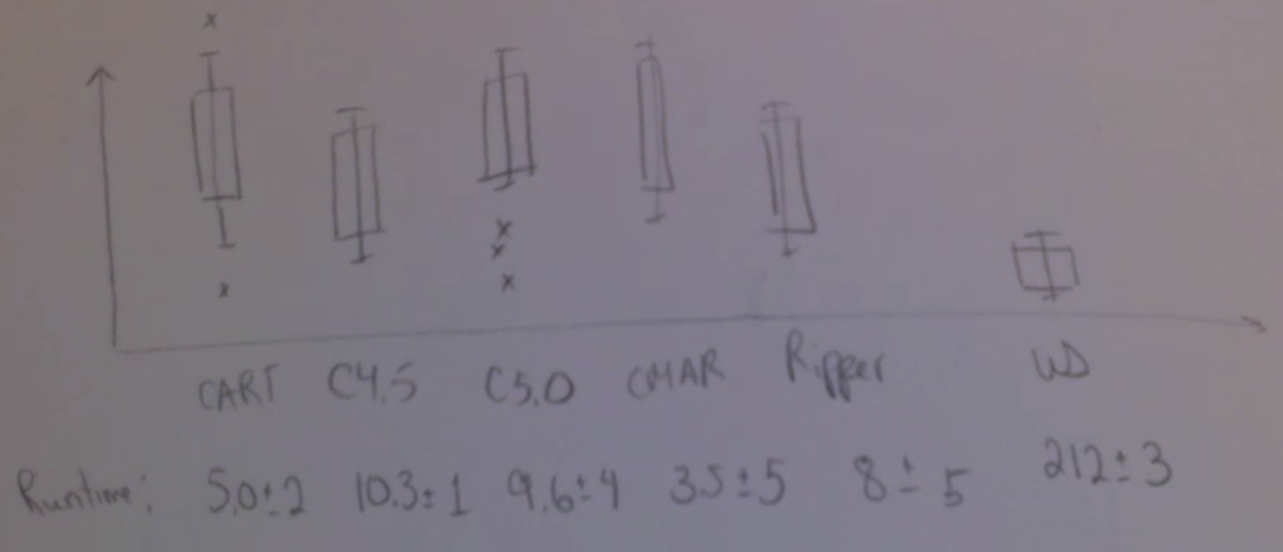
\includegraphics[width=0.75\textwidth]{figs/sketch-comparison.png}
\end{center}
\caption{Comparison with other methods:
Value of the objective for us and a few other algorithms
(CART, C4.5, CBA, CMAR/CPAR, C5.0, Ripper, \dots), and algorithm runtimes,
over ten folds, for one big dataset (box plots)}
\label{fig:comparison}
\end{figure}

\begin{figure}[t!]
\begin{center}
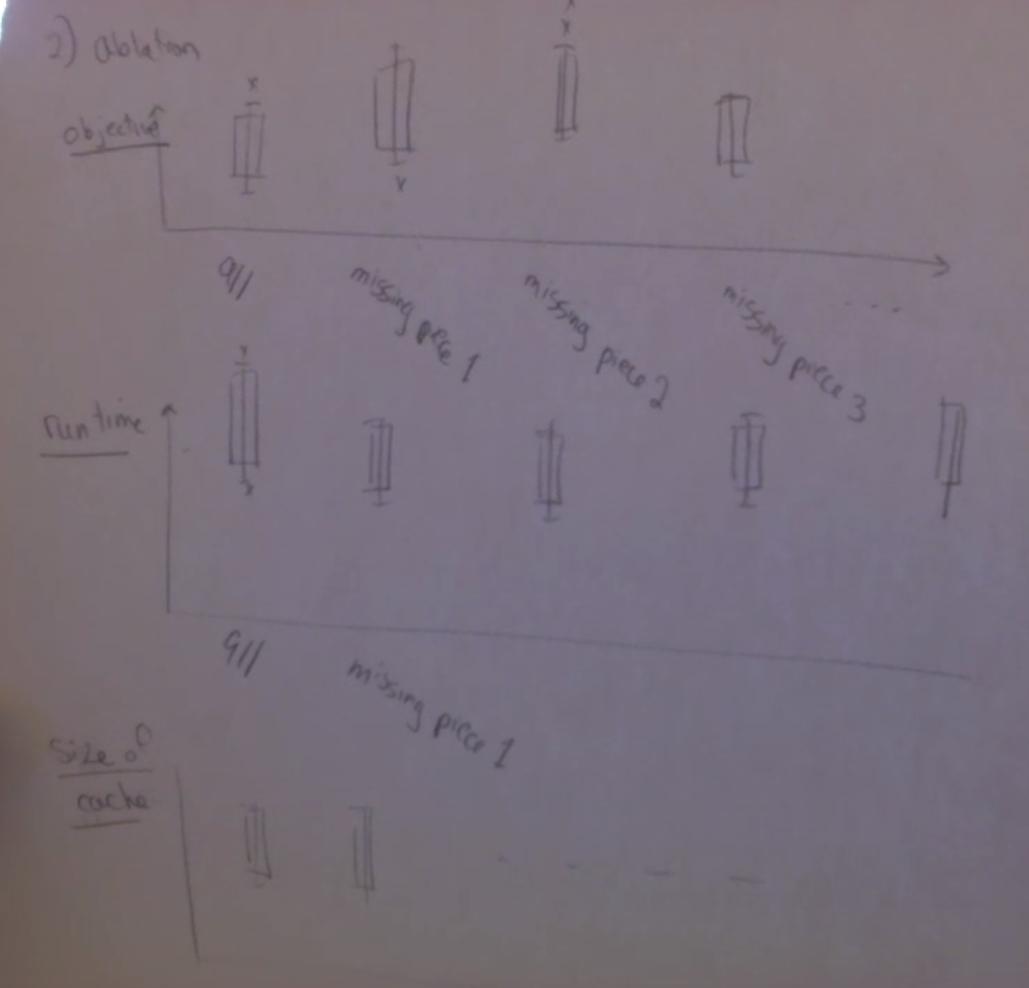
\includegraphics[width=0.75\textwidth]{figs/sketch-ablation.png}
\end{center}
\caption{Ablation experiment:
Show the effect of each ``piece'' at a time,
run X without each in turn and show the difference in either
quality of solution or runtime or amount of memory, size of cache or queue,
where X is a specific implementation
(meaning a specific scheduling policy and node type)}
\label{fig:ablation}
\end{figure}

\begin{figure}[t!]
\begin{center}
\end{center}
\caption{Missing:  Some sort of comparison of different scheduling policies}
\label{fig:scheduling-policy}
\end{figure}

\begin{figure}[t!]
\begin{center}
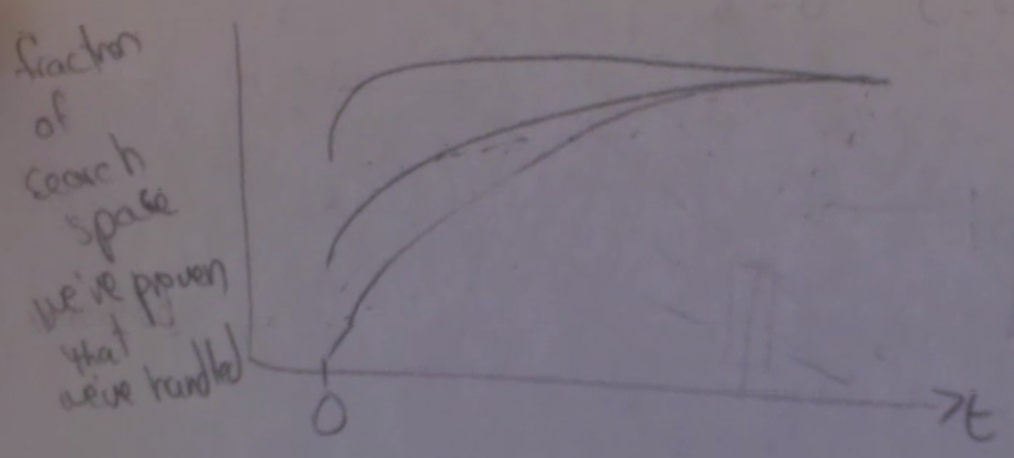
\includegraphics[width=0.65\textwidth]{figs/sketch-search-space.png}
\end{center}
\caption{Fraction of search space we've proven we've handled}
\label{fig:search-space}
\end{figure}

\begin{figure}[t!]
\begin{center}
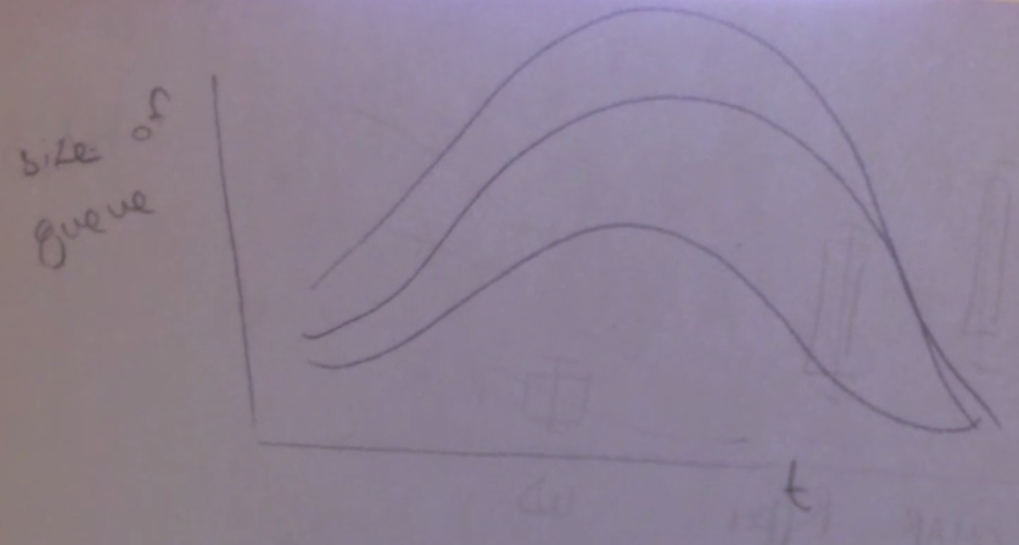
\includegraphics[width=0.65\textwidth]{figs/sketch-queue-size.png}
\end{center}
\caption{Size of queue over time}
\label{fig:queue-size}
\end{figure}

\begin{figure}[t!]
\begin{center}
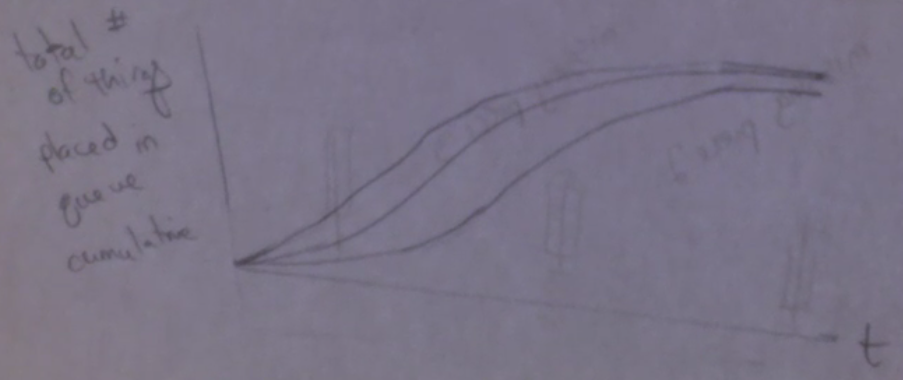
\includegraphics[width=0.65\textwidth]{figs/sketch-queue-cumulative.png}
\end{center}
\caption{Cumulative number of things placed in queue over time}
\label{fig:queue-cumulative}
\end{figure}

\begin{figure}[t!]
\begin{center}
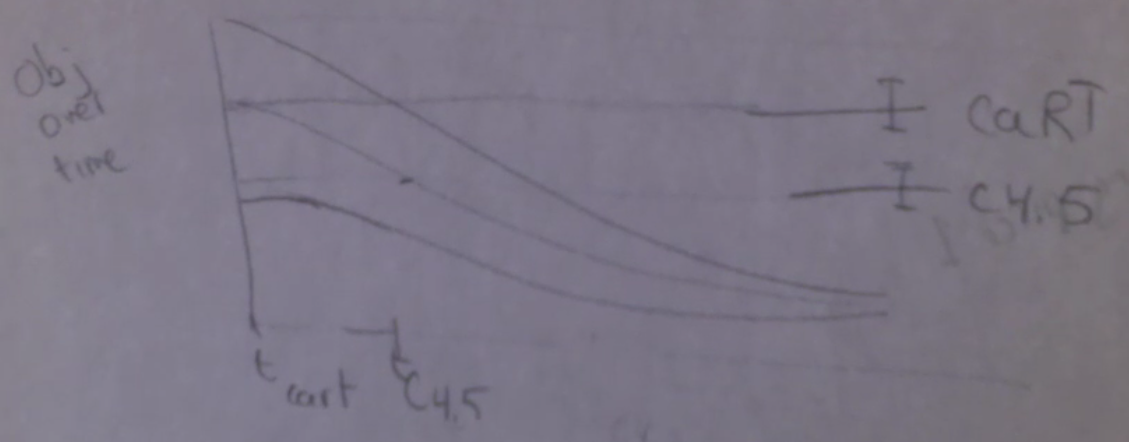
\includegraphics[width=0.65\textwidth]{figs/sketch-objective.png}
\end{center}
\caption{Objective value over time,
with horizontal lines and x-ticks for CART and C4.5}
\label{fig:objective}
\end{figure}

\begin{figure}[t!]
\begin{center}
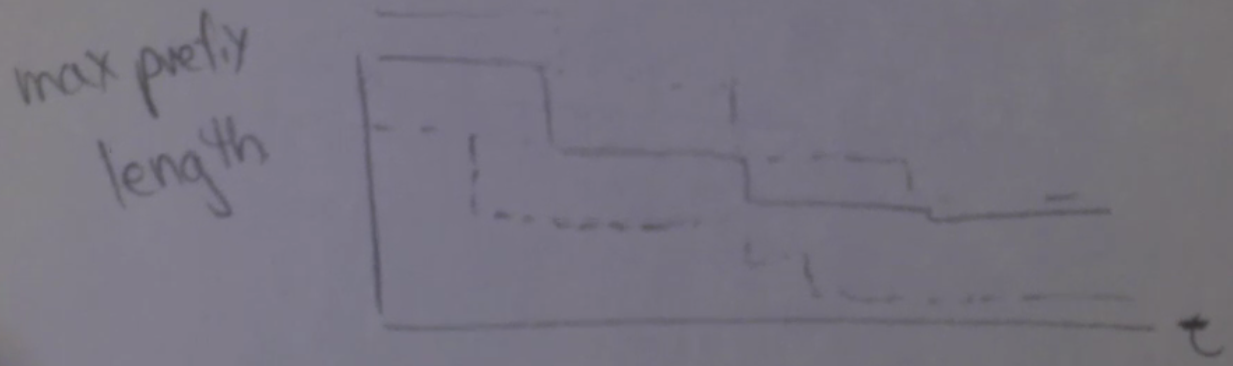
\includegraphics[width=0.65\textwidth]{figs/sketch-max-length.png}
\end{center}
\caption{Max prefix length over time (computed from objective value);
maybe also add the best prefix length over time}
\label{fig:max-length}
\end{figure}
